%%%%%%%%%%%%%%%%%%%%%%%%%%%%%%%%%%%%%%%%%%%%%%%%%%%%%%%%%%%%%%%%%%%%%%%%%%%%%%%
%                                                                             %
% 02 - Marco Teórico                                                          %
%                                                                             %
%%%%%%%%%%%%%%%%%%%%%%%%%%%%%%%%%%%%%%%%%%%%%%%%%%%%%%%%%%%%%%%%%%%%%%%%%%%%%%%

\chapter{\textcolor{azulescom}{Marco teórico}}

\section{Valuación Inmobiliaria}
La \gls{valuacion} inmobiliaria es el proceso mediante el cual se determina el valor
de un bien inmueble, es decir, el precio estimado en que podría ser vendido o
comprado. Para esto, se toman en cuenta las características físicas,
económicas, sociales y legales del inmueble, así como las condiciones del
mercado inmobiliario en el que se encuentra.

Un bien \gls{inmueble} se define como: ``... todos los intereses, beneficios, derechos y
gravámenes inherentes a la propiedad de bienes raíces físicos, donde los bienes
raíces son la tierra junto con todas las mejoras que están permanentemente
adheridas a ella y todos los accesorios asociados a la misma" \cite{pagourtzi2003}.
La Consejería Jurídica del Gobierno de la Ciudad de México, por su parte, define
a los inmuebles como: ``... aquella cosa que no puede trasladarse de un lugar a
otro, por ejemplo, un terreno o edificio.'' \cite{cdmx2014inmueble}.

A pesar de que existen múltiples criterios de clasificación de los bienes inmuebles,
en la práctica se utilizan dos criterios principales: el uso y la naturaleza del
inmueble. El criterio de uso se refiere a la función que cumple el inmueble,
mientras que el criterio de naturaleza se refiere a las características físicas
del inmueble. Así, para fines de este trabajo terminal, se considerarán los bienes
inmobiliarios de tipo de uso \textit{multifamiliar} y de tipo de naturaleza
\textit{desarrollos inmobiliarios verticales}, mejor conocidos como \textit{departamentos}.

\subsection{Importancia de la valuación inmobiliaria}
El proceso de valuación inmobiliaria es requerido para tener una medida cuantitativa
de los beneficios y riesgos de poseer un bien inmueble. Es decir, permite
determinar el valor de un bien inmueble, el cual es un factor determinante en
la toma de decisiones de inversión, financiamiento, compra, venta, arrendamiento,
entre otras.

Algunos de los jugadores clave en el proceso de valuación inmobiliaria son
\cite{pagourtzi2003}:

\begin{itemize}
  \item \textbf{Agentes inmobiliarios:} Son los encargados de la promoción y
  venta de bienes inmuebles.
  \item \textbf{Valuadores:} Son personas especializadas en la valuación de
  bienes inmuebles, generalmente realizando inspecciones físicas y análisis
  de mercado.
  \item \textbf{Asesores financieros:} Son aquellos individuos especializados
  en el análisis de la situación financiera de una persona o empresa, con el
  fin de recomendar las mejores opciones de inversión, financiamiento, compra,
  venta, arrendamiento, entre otras.
  \item \textbf{Instituciones financieras:} Son aquellas instituciones que
  ofrecen servicios y productos financieros, como créditos hipotecarios,
  préstamos, entre otros.
  \item \textbf{Desarrolladores inmobiliarios:} Se refiere a las personas u
  organizaciones que se dedican a la construcción de bienes inmuebles.
  \item \textbf{Inversionistas:} Son aquellas personas o grupos empresariales
  que realizan inversiones en bienes inmuebles o desarrollos inmobiliarios con
  el fin de obtener un beneficio económico.
  \item \textbf{Analistas de mercado:} Son personas especializadas en el
  análisis de las condiciones del mercado inmobiliario, con el fin de
  determinar las tendencias y proyecciones del mismo.
  \item \textbf{Gobierno:} Se refiere a las instituciones gubernamentales y
  mecanismos de gobierno que regulan el mercado inmobiliario.
\end{itemize}

\subsection{Valuación inmobiliaria en México}
En México la valuación de bienes nacionales están regulados por la Secretaría de
Economía mediante la norma oficial mexicana NMX-C-459-SCFI-ONNCCE-2007
\cite{nmx-c-459-scfi-onncce-2007}, los cuales son generalmente administrados por
el \acrfull{indaabin}. A pesar de que en su primer implementación en 2007 no se
tenía un equivalente internacional, recientemente esta norma
fue compatibilizada con la provista por el \acrfull{ivsc}. En esta norma se establecen los
requisitos mínimos que deben cumplir los valuadores para realizar una valuación
inmobiliaria, así como los requisitos mínimos que debe cumplir un reporte de
valuación inmobiliaria. La misma Secretaría de Economía, a través de la \acrfull{shn},
establece las ``Reglas de carácter general que establecen la metodología para la
valuación de inmuebles" \cite{salas2014valuacion}.

Por su parte, la \acrfull{cnbv} establece los criterios para la valuación de
inmuebles que sirven como garantía de créditos otorgados por las instituciones
de crédito \cite{cnbv2023}.

En el caso de la Ciudad de México, la \acrfull{sedeco} ofrece dos certificaciones
en materia de valuación inmobiliaria\cite{inmuebles24certificacion}:

\begin{itemize}
  \item \textbf{Corredor Inmobiliario}: es la persona física que se dedica a los
  temas legales y financieros de la compraventa de bienes inmuebles.
  \item \textbf{Administrador Inmobiliario}: es la persona que se especializa
  en los aspectos fiscales, tributarios y administrativos de los bienes inmuebles.
\end{itemize}

\subsection{Métodos de valuación inmobiliaria tradicionales}
Existen múltiples métodos de valuación inmobiliaria, los cuales se pueden
clasificar en tres categorías principales: métodos basados en el mercado,
métodos basados en el ingreso y métodos basados en el costo. En la práctica,
los métodos basados en el mercado son los más utilizados, ya que son los que
requieren de menor información y son más fáciles de implementar. Sin embargo,
los métodos basados en el ingreso y en el costo son utilizados cuando no se
cuenta con información suficiente del mercado inmobiliario \cite{mexhome2021}.

Existen múltiples regulaciones y criterios en relación a la valuación inmobiliaria,
y dependerá del objetivo de la misma la regulación a acatar y el método disponible
a utilizar. En el cuadro \ref{tab:metodos-valuacion-tradicional} se muestran los
métodos de valuación inmobiliaria tradicionales más utilizados en México \cite{mexhome2021}.

\begin{table}[h]
  \centering
  \caption{Métodos de Valuación Inmobiliaria Tradicionales en México}
  \begin{tabular}{|p{4cm}|p{5cm}|p{3cm}|}
  \hline
  \rowcolor{azulclaro}
  \centering\textbf{Método} & \centering\textbf{Descripción} & \centering\textbf{Aplicación}\arraybackslash \\
  \hline
  Enfoque de Comparación de Ventas & Compara la propiedad con otras similares que se hayan vendido recientemente en la misma zona. Basado en el supuesto de que propiedades con características similares deberían tener valores similares. & Ampliamente utilizado en México para todo tipo de propiedades. \\
  \hline
  Enfoque de Costos & Estima el coste de construcción de un \gls{inmueble} similar a partir de cero y deduce la depreciación. Basado en el supuesto de que el valor de una propiedad viene determinado por el coste de su sustitución. & Utilizado para propiedades nuevas o recientemente renovadas. \\
  \hline
  Enfoque Basado en los Ingresos & Estima los ingresos que probablemente generará el \gls{inmueble} a lo largo de su vida útil. Basado en el supuesto de que el valor de una propiedad comercial viene determinado por su potencial de generación de ingresos. & Utilizado para valorar inmuebles comerciales. \\
  \hline
  \end{tabular}
  \label{tab:metodos-valuacion-tradicional}
\end{table}

\subsection{Retos y limitantes de la valuación inmobiliaria tradicional en México}
A pesar de que los métodos de valuación inmobiliaria tradicionales son socorridos
por múltiples actores e instituciones del sector inmobiliario, el \acrfull{bid}
ha identificado múltiples retos y limitantes en su implementación desde una
perspectiva catastral \cite{eguino2020catastro}. Entre los retos y limitantes
se encuentran:

\begin{itemize}
  \item \textbf{Falta de información:} La información catastral es limitada y
  no se encuentra disponible en formatos digitales, lo que dificulta su
  procesamiento y análisis.
  \item \textbf{Falta de estandarización:} La información catastral no se
  encuentra estandarizada, lo que dificulta su procesamiento y análisis.
  \item \textbf{Falta de transparencia:} La información catastral no se
  encuentra disponible para el público en general, lo que dificulta su
  procesamiento y análisis.
  \item \textbf{Falta de actualización:} La información catastral no se
  encuentra actualizada, lo que dificulta su procesamiento y análisis.
  \item \textbf{Falta de integración:} La información catastral no se
  encuentra integrada con otras fuentes de información, lo que dificulta su
  procesamiento y análisis.
\end{itemize}

Además, para determinar si uno los métodos de valuación tradicionales ofrece resultados
confiables, en el año 1999 se llevó a cabo un estudio en el que se compararon
múltiples mecanismos de valuación y se analizaron los resultados obtenidos. La
conclusión es que la valuación posee inherentemente un alto grado de subjetividad
y, a pesar de que existen mecanismos como \acrfull{deps} que buscan minimizar y
compensar el error, su implementación es sumamente compleja ya que requiere de
una gran cantidad de consideraciones y supuestos que deben ser tomados en cuenta
\cite{Shiller:1999aa}.

\subsection{Inteligencia Artificial en la valuación inmobiliaria}
A fin de poder ofrecer una valuación inmobiliaria que sea confiable, se requiere
del uso de estrategias que permitan minimizar el error a la vez que se consideran
e integran múltiples fuentes de información. En este sentido, la \acrfull{ia}
ha demostrado ser más flexible para resolver problemas de prediccion de valores
de mercado que otros enfoques metodológicos \cite{eguino2020catastro}.

En particular, los modelos de valuación automática (\acrfull{avm}, por sus siglas en inglés) basados en \acrshort{ia}
han demostrado ser más precisos que los métodos tradicionales de valuación
inmobiliaria \cite{eguino2020catastro}. Dentro de los \acrshort{avm}
se destecan los métodos basados en \acrfull{rna}, precios hedónicos, análisis
geoespacial, lógica difusa y \acrfull{arima} \cite{pagourtzi2003}.

\section{Inteligencia Artificial}
La inteligencia artificial (IA) se define como la ciencia e ingeniería de crear
máquinas inteligentes, particularmente programas de computadora inteligentes.
Aunque está relacionada con la tarea de usar computadoras para comprender la
inteligencia humana, la IA no se limita a métodos que son biológicamente observables.
La inteligencia, en este contexto, se refiere a la parte computacional de la
capacidad para lograr objetivos en el mundo, la cual varía en personas, muchos
animales y algunas máquinas. Hasta ahora, no existe una definición sólida y
universal de inteligencia que sea independiente de la inteligencia humana,
principalmente porque aún no se caracterizan en general los procedimientos
computacionales que se quieren calificar como inteligentes. La IA implica
mecanismos que han sido parcialmente descubiertos por la investigación,
permitiendo a las computadoras realizar algunas tareas con gran eficacia,
mientras que otras aún no están al alcance. La IA no siempre busca simular
la inteligencia humana; en muchas ocasiones, se centra más en resolver problemas
presentados por el mundo que en imitar a las personas o animales. Esto permite a
los investigadores de IA utilizar métodos que no se observan en humanos o que
requieren más capacidad de cómputo de la que los humanos pueden realizar. La IA
actual se caracteriza por tener mucha velocidad y memoria, pero sus habilidades
se limitan a los mecanismos intelectuales que los diseñadores de programas
comprenden lo suficiente como para implementar en programas. La inteligencia
artificial es un campo en constante evolución, buscando alcanzar niveles de
inteligencia comparables a los humanos, aunque esto aún parece requerir ideas
fundamentales nuevas y una comprensión más profunda de los mecanismos de la
inteligencia \cite{mccarthy2004artificial}.

\subsection{Aprendizaje Automático}
El aprendizaje se refiere a un amplio espectro de situaciones en las cuales el
aprendiz incrementa su conocimiento o sus habilidades para cumplir una tarea. El aprendizaje
aplica inferencias a determinada información para construir una representación apropiada de
algú aspecto relevante de la realidad o de algún proceso \cite{moreno1994aprendizaje}.
En la Figura \ref{fig:aprendizaje} se muestra un diagrama general de aprendizaje
automático y sus componentes.

\begin{figure}[!htbp]
  \centering
  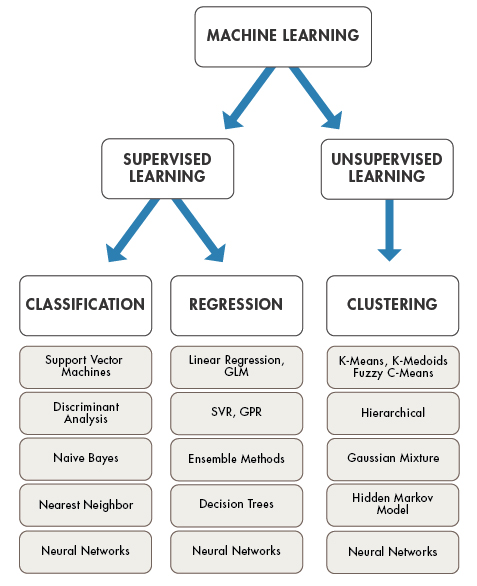
\includegraphics[width=0.4\textwidth]{imagenes/02-marco-teorico/machinelearningtypes.jpg}
  \caption[Diagrama de Aprendizaje Automático]{Diagrama general de algoritmos de Aprendizaje Automático \cite{mathworks_machine_learning}.}
  \label{fig:aprendizaje}
\end{figure}


\subsection{Aprendizaje Supervisado}
El aprendizaje supervisado implica aprender un mapeo entre un conjunto de
variables de entrada \( \mathbf{X} \) y una variable de salida \( Y \), y
aplicar este mapeo para predecir las salidas de datos no vistos. El aprendizaje
supervisado es la metodología más importante en el aprendizaje automático y
también tiene una importancia central en el procesamiento de datos inmobiliarios.
En este capítulo, nos centramos en enfoques basados en kernels para el
aprendizaje supervisado. Revisamos las máquinas de vectores de soporte,
que representan la tecnología de aprendizaje supervisado dominante en la
actualidad, particularmente en el procesamiento de datos multimedia. También
revisamos los clasificadores de vecinos más cercanos que pueden considerarse,
en términos generales, una estrategia basada en kernel. Las técnicas de vecinos
más cercanos son populares en valuaciones porque el énfasis en la similitud es
apropiado para múltiples contextos \cite{Cunningham2008}.

En el Cuadro \ref{table:comparativa-algoritmos-supervisado} se muestra una
comparativa de los algoritmos de aprendizaje supervisado más utilizados en la
actualidad, así como sus ventajas, desventajas y librerías disponibles en Python
\cite{10.1145/1143844.1143865}.


\begin{table}[h]
\centering
\tiny
\begin{tabular}{|l|p{2cm}|p{2.5cm}|p{2.5cm}|p{1.5cm}|}
\hline
\rowcolor{azulclaro}
\textbf{Nombre} & \textbf{Descripción} & \textbf{Ventajas} & \textbf{Desventajas} & \textbf{Librería Python} \\ \hline
Regresión Logística & Clasificación lineal. & Interpretable, simple. & Limitada en complejidad. & \texttt{sklearn} \\ \hline
SVMs & Alto rendimiento en espacios dimensionales. & Bueno para muchas dimensiones. & Selección de kernel crucial. & \texttt{sklearn} \\ \hline
Decision Trees & Estructura en forma de árbol. & Fácil interpretación. & Riesgo de sobreajuste. & \texttt{sklearn} \\ \hline
Random Forests & Conjunto de árboles. & Reduce sobreajuste. & Menos interpretable. & \texttt{sklearn} \\ \hline
Naive Bayes & Basado en teorema de Bayes. & Eficiente y sencillo. & Suposiciones de independencia. & \texttt{sklearn} \\ \hline
Neural Networks & Modelos tipo cerebro. & Muy flexibles. & Tiempo de entrenamiento. & \texttt{tensorflow}, \texttt{keras} \\ \hline
Memory-Based & Aprendizaje por instancias. & No necesita modelo. & Ineficiente en grandes datos. & \texttt{sklearn} \\ \hline
Bagged Trees & Árboles ensacados. & Menor varianza. & Menor interpretabilidad. & \texttt{sklearn} \\ \hline
Boosted Trees & Árboles potenciados. & Alta eficacia en clasificación. & Riesgo de sobreajuste. & \texttt{xgboost} \\ \hline
Boosted Stumps & Tocones potenciados. & Bueno para datos dimensionales. & Menos potentes que árboles. & \texttt{xgboost} \\ \hline
\end{tabular}
  \caption{Comparativa de algoritmos de aprendizaje supervisado \cite{10.1145/1143844.1143865}.}
\label{table:comparativa-algoritmos-supervisado}
\end{table}

\subsubsection{Máquinas de Soporte Vectorial}
Método efectivo en espacios de alta dimensión. Utiliza hiperplanos para separar
clases de datos. Los hiperplanos se eligen maximizando el margen entre las clases.
Las SVMs pueden usar diferentes tipos de kernels, como lineal, polinomial y
radial, para adaptarse a la naturaleza no lineal de algunos datos \cite{10.1145/1143844.1143865}.

\subsubsection{Bosques Aleatorios}
Método de ensamblaje que utiliza múltiples árboles de decisión para mejorar la
robustez y precisión. Cada árbol se entrena con una muestra aleatoria del
conjunto de datos. La decisión final se toma por votación mayoritaria o
promediando las salidas de todos los árboles. Efectivo para reducir el sobreajuste
en comparación con un solo árbol de decisión \cite{10.1145/1143844.1143865}.

\subsubsection{Redes Neuronales Artificiales}
Las \acrfull{rna} son sistemas adaptativos inspirados en
cómo funciona el cerebro humano, con la capacidad de modificar su estructura
interna para alcanzar un objetivo específico. Son especialmente útiles para
resolver problemas no lineales, logrando descifrar las reglas difusas que rigen
las soluciones óptimas para estos. Compuestas por nodos o elementos de
procesamiento (PE), cada uno con su entrada y salida, permiten la
intercomunicación entre ellos y con el entorno \cite{grossi2007introduction}.
En la Figura \ref{fig:neurona} se muestra una neurona biológica, la cual es la
inspiración de la unidad básica de procesamiento de una \acrshort{rna}.

\begin{figure}[!htbp]
  \centering
  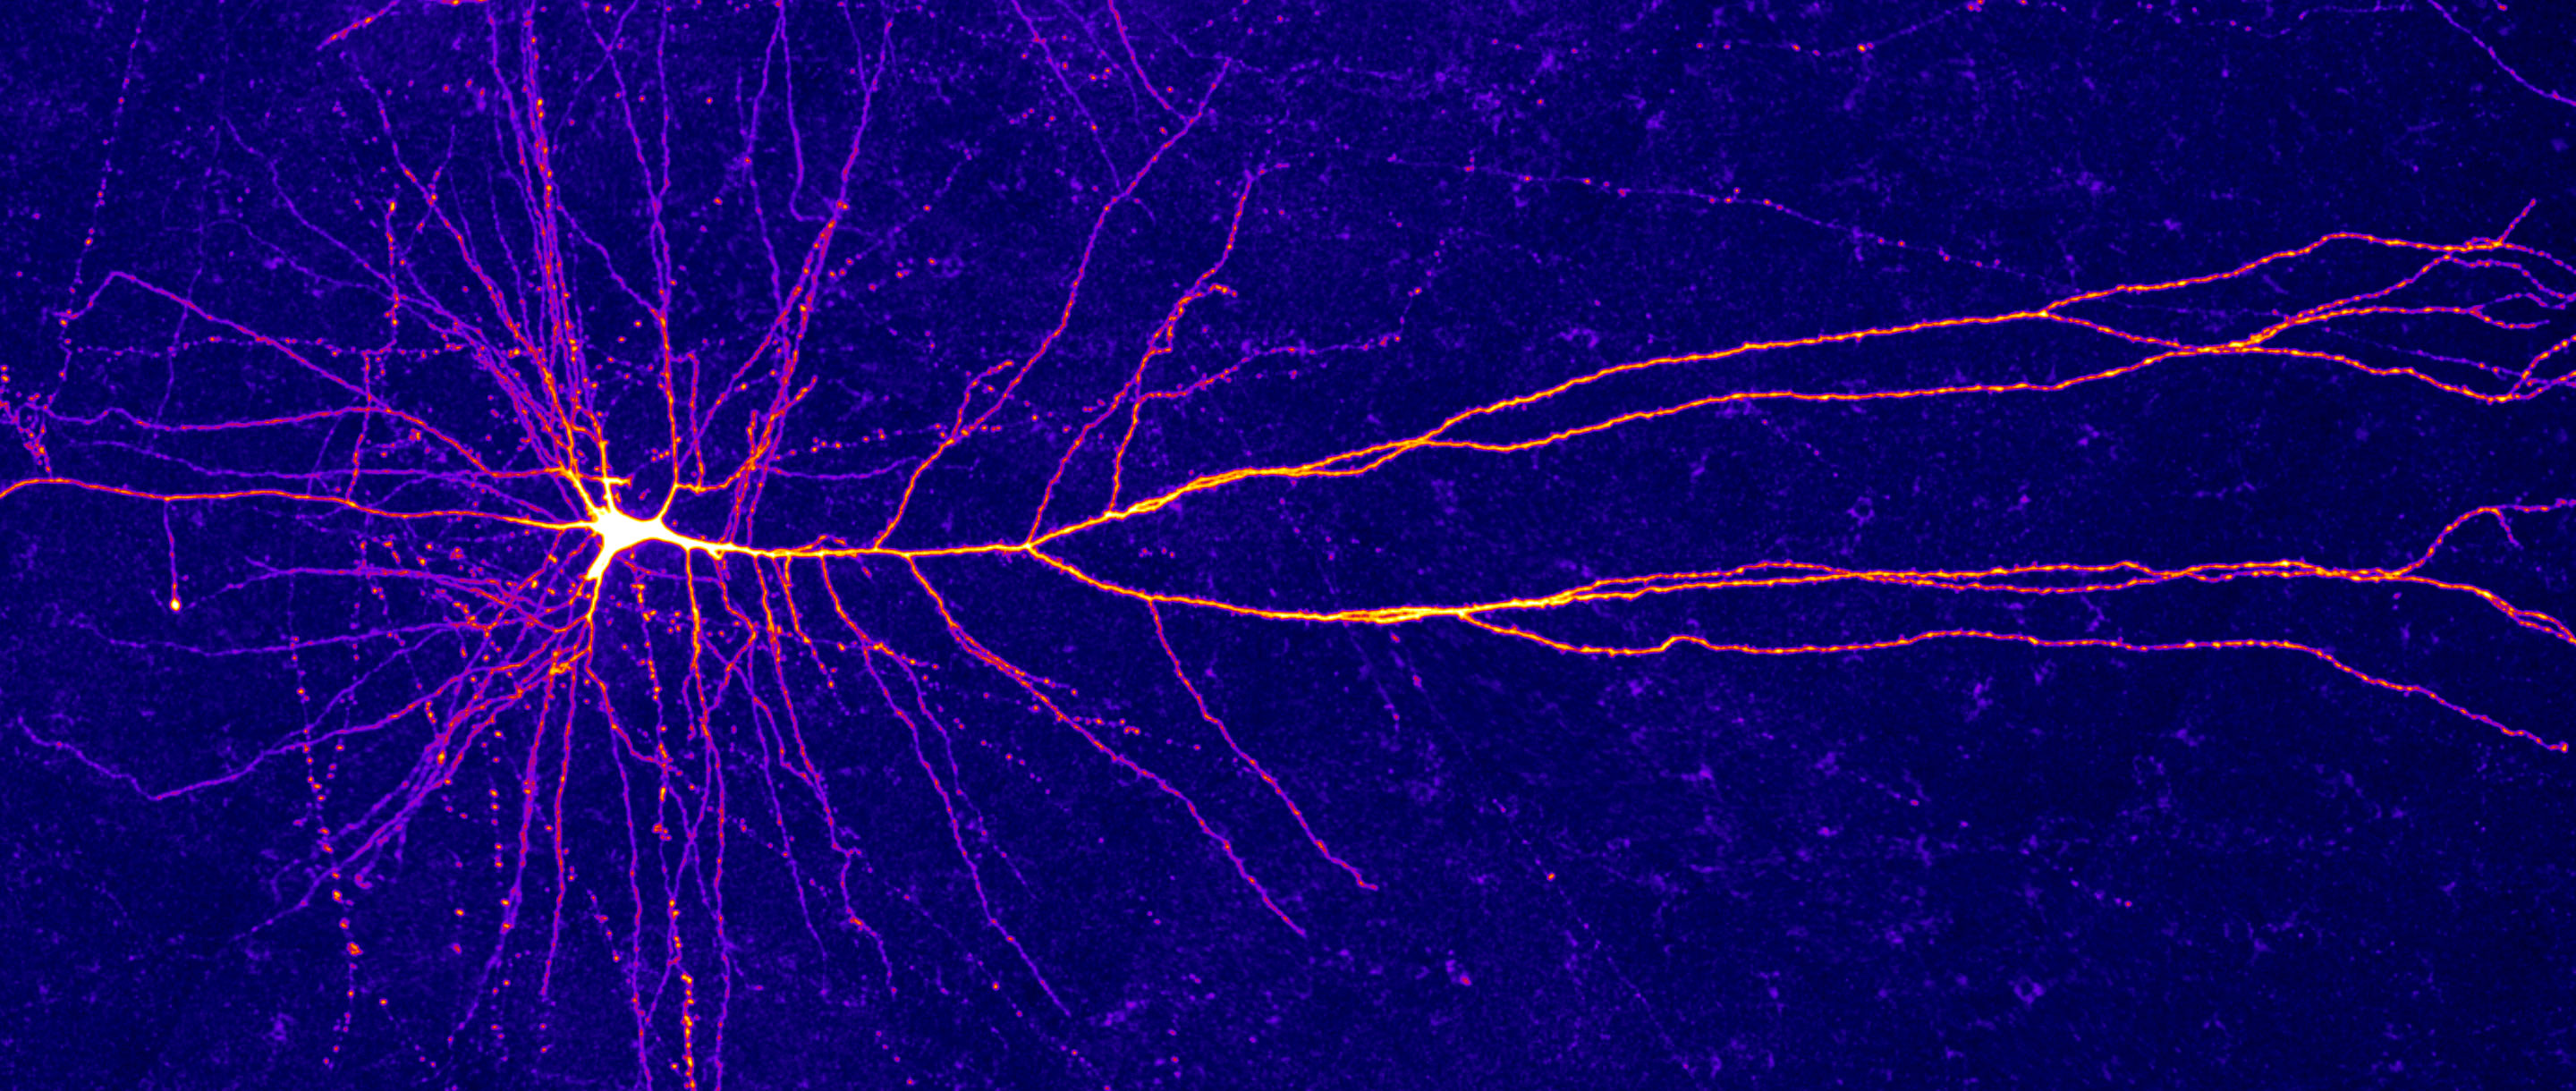
\includegraphics[width=0.9\textwidth]{imagenes/02-marco-teorico/red-neuronal-dendritas.jpg}
  \caption[Neurona]{Neurona \cite{vida_neurocure_2020}}
  \label{fig:neurona}
\end{figure}

Una red neuronal artificial está compuesta por múltiples capas de nodos, cada
una de las cuales está conectada con la siguiente. La primera capa se conoce como
capa de entrada, la última como capa de salida y las capas intermedias como capas
ocultas. Cada nodo de una capa está conectado con todos los nodos de la capa
siguiente, pero no con los de la misma capa. Cada conexión entre nodos tiene un
peso asociado, el cual se utiliza para determinar la salida de un nodo \cite{ibm2023redneuronal}. La
figura \ref{fig:red-neuronal-ibm} muestra un ejemplo de una red neuronal artificial.

\begin{figure}[!htbp]
  \centering
  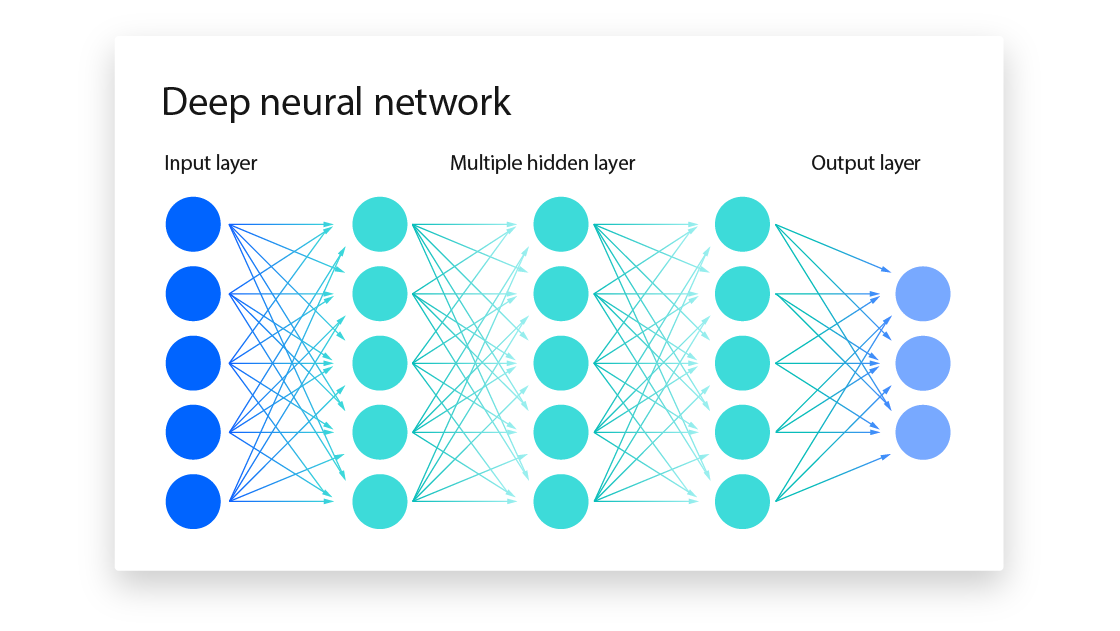
\includegraphics[width=0.9\textwidth]{imagenes/02-marco-teorico/red-neuronal-ibm.png}
  \caption[Red Neuronal]{Red Neuronal \cite{ibm2023redneuronal}}
  \label{fig:red-neuronal-ibm}
\end{figure}

\subsection{Librerías de Aprendizaje Automático en Python}

Para realizar la implementación de alguno de los algoritmos de aprendizaje
mencionados anteriormente, se requiere de librerías que implementen dichos
algoritmos para facilitar su uso. Esto resulta en un ahorro de tiempo y esfuerzo
para el desarrollador, ya que no es necesario implementar los algoritmos desde
cero y se tiene certeza sobre la calidad de los mismos. En el caso de Python,
existen múltiples librerías que implementan los algoritmos de aprendizaje
automático más utilizados en la actualidad. En esta sección se describen las
librerías con mayor popularidad y que son utilizadas en el presente trabajo
terminal.

\subsubsection{Scikit-Learn}

Scikit-learn es un módulo de Python que integra una amplia gama de algoritmos
de aprendizaje automático de última generación para problemas supervisados y no
supervisados de escala media. Este paquete se centra en llevar el aprendizaje
automático a los no especialistas utilizando un lenguaje de alto nivel de propósito
general. Se pone énfasis en la facilidad de uso, el rendimiento, la documentación
y la consistencia de la API. Tiene dependencias mínimas y se distribuye bajo la
licencia BSD simplificada, fomentando su uso tanto en entornos académicos como
comerciales \cite{pedregosa2011scikit}.

\begin{figure}[!htbp]
  \centering
  
\includegraphics[width=0.3\textwidth]{imagenes/02-marco-teorico/scikit-logo.png}
  \caption[Logo de Scikit-Learn]{Logo de Scikit-Learn \cite{scikit-learn}}
  \label{fig:scikit-learn-logo}
\end{figure}

\subsubsection{TensorFlow}

TensorFlow es un sistema de aprendizaje automático que opera a gran escala y en
entornos heterogéneos. Su modelo computacional se basa en grafos de flujo de
datos con estado mutable. Los nodos del grafo pueden mapearse a diferentes
máquinas en un clúster, y dentro de cada máquina a CPUs, GPUs y otros
dispositivos. TensorFlow admite una variedad de aplicaciones, pero se enfoca
particularmente en el entrenamiento y la inferencia con redes neuronales
profundas. Sirve como plataforma tanto para la investigación como para la
implementación de sistemas de aprendizaje automático en muchas áreas, tales
como reconocimiento de voz, visión por computadora, robótica, recuperación de
información y procesamiento de lenguaje natural. En esta charla, describimos
TensorFlow y esbozamos algunas de sus aplicaciones. También discutimos la
cuestión de qué relación puede tener TensorFlow y el aprendizaje profundo con
la programación funcional. Aunque TensorFlow no es puramente funcional, muchos
de sus usos están relacionados con la optimización de funciones (durante el
entrenamiento), y luego con la aplicación de esas funciones (durante la
inferencia). Estas funciones se definen como composiciones de primitivas
simples (como es común en la programación funcional), con representaciones
internas de datos que se aprenden en lugar de diseñarse manualmente. TensorFlow
es un trabajo conjunto con muchas otras personas del equipo de Google Brain y
otros lugares \cite{abadi2016tensorflow}.

\begin{figure}[!htbp]
  \centering
  
\includegraphics[width=0.3\textwidth]{imagenes/02-marco-teorico/tensorflow-logo.png}
  \caption[Logo de TensorFlow]{Logo de TensorFlow \cite{abadi2016tensorflow}}
  \label{fig:tensorflow-logo}
\end{figure}

\subsubsection{Keras}
Keras es una API de aprendizaje profundo escrita en Python, que se ejecuta sobre
TensorFlow, una plataforma de aprendizaje automático. Fue desarrollada con el
objetivo de facilitar la experimentación rápida, permitiendo a los usuarios
pasar de la idea al resultado de manera ágil, lo cual es fundamental para
realizar una buena investigación. Las características principales de Keras son su simplicidad, flexibilidad y
potencia.Keras reduce la carga cognitiva
del desarrollador, permitiéndole concentrarse en los aspectos más importantes
del problema. Su diseño flexible se basa en el principio de revelación
progresiva de la complejidad: los flujos de trabajo simples deben ser rápidos
y fáciles de implementar, mientras que los flujos de trabajo avanzados deben
ser posibles mediante un camino claro que se apoya en los conocimientos previos
del usuario. En cuanto a potencia, Keras ofrece un rendimiento y una escalabilidad
de nivel industrial, siendo utilizada por organizaciones y empresas de renombre,
incluyendo NASA, YouTube y Waymo. Esto subraya su capacidad para manejar
proyectos de aprendizaje profundo a gran escala y con requerimientos complejos \cite{keras}.

\begin{figure}[!htbp]
  \centering
  
\includegraphics[width=0.3\textwidth]{imagenes/02-marco-teorico/keras-logo.png}
  \caption[Logo de Keras]{Logo de Keras \cite{keras}}
  \label{fig:keras-logo}
\end{figure}

\section{Conjunto de Datos}
Para poder realizar el entrenamiento de un modelo de \acrshort{rna} se requiere
de un conjunto de datos (\gls{dataset}) que contenga información histórica de
los inmubles a evaluar \cite{pagourtzi2003}. Dentro de las opciones que tenemos para obtener un
\gls{dataset} se encuentran:

\begin{itemize}
  \item \textbf{Construir un \gls{dataset} propio:} Se requeriría de un formulario
  para recabar información y de un mecanismo para almacenarla. Sin embargo,
  la cantidad de información sería mínima y no nos permitiría obtener un modelo
  representativo del mercado en cuestión.
  \item \textbf{Utilizar un \gls{dataset} existente:} En este punto se podrían
  utilizar los datos del catastro, o aquellos disponibles de alguna investigación
  similar previa. El problema con usar los valores catastrales es que no son
  confiables (en términos de precios de mercado) y están sujetos a múltiples
  factores que no son considerados en la valuación inmobiliaria tradicional \cite{eguino2020catastro}.
  Referente a investigaciones previas, los datos que pudieron observarse están
  desactualizados (no representan un valor de mercado actualizado), o bien, no
  se encuentran disponibles para la Ciudad de México y corresponden a otras
  ciudades del país.
  \item \textbf{Obtener un \gls{dataset} mediante \textit{Web Scraping}:} En este
  caso, se crearía un \gls{dataset} a partir de la información disponible en
  algún portal inmobiliario. Para esto, se requiere de la construcción de un
  \textit{web scraper} el cual permita extraer la información de interés y la
  almacene en una base de datos. El problema sería realizar la limpieza de los
  datos obtenidos a bien de no entrenar el modelo con información errónea.
\end{itemize}

\subsection{Conjuntos de Datos ya existentes}

Con el objetivo de encontrar un conjunto de datos que pudiera ser utilizado
para el entrenamiento de un modelo de regresión, se realizó una búsqueda en
diferentes plataformas de datos abiertos. En la Figura \ref{fig:catastro-cdmx}
se muestra el único conjunto encontrado que contiene información de la Ciudad
de México, el cual corresponde a los valores catastrales de la Ciudad de México.

\begin{figure}[!htbp]
  \centering
  
\includegraphics[width=0.9\textwidth]{imagenes/02-marco-teorico/catastro-cdmx.png}
  \caption[Conjunto de Datos del Catastro de la Ciudad de México]{Conjunto de Datos del Catastro de la Ciudad de México \cite{sigcdmx}.}
  \label{fig:catastro-cdmx}
\end{figure}

\subsubsection{Datos Catastrales de la Ciudad de México}

A pesar de que el conjunto de datos del catastro de la Ciudad de México es el
único \gls{dataset} que contiene información de la Ciudad de México, existen
múltiples limitantes que impiden su uso para el entrenamiento de un modelo de
\acrshort{rna}:

Los datos catastrales a menudo no reflejan las condiciones actuales del
mercado inmobiliario. El catastro se enfoca en la descripción física y la
ubicación de la propiedad, pero generalmente no actualiza los valores de manera
frecuente para reflejar las tendencias actuales del mercado. Esto significa que
los precios catastrales pueden estar desactualizados y no coincidir con los
precios de mercado reales, que son influenciados por factores dinámicos como la
demanda y oferta actual, el estado económico general, y las tendencias específicas
de la zona \cite{eguino2020catastro}.

Por otro lado, los valores catastrales a menudo se calculan con fines fiscales
y pueden estar basados en criterios que no necesariamente coinciden con los que
determinan el valor de mercado de una propiedad. Por ejemplo, un catastro puede
valorar las propiedades basándose en su tamaño y ubicación, pero no necesariamente
toma en cuenta factores como el estado de la propiedad, las mejoras realizadas, o
características únicas que podrían aumentar su valor de mercado. Además, en
algunos casos, los valores catastrales pueden estar influenciados por políticas
fiscales, lo que podría llevar a una subestimación o sobreestimación del valor
real del inmueble en el mercado \cite{sigcdmx}.

\subsection{Web Scraping}
El \textit{web scraping} es la técnica en la que se extraen datos de una o varias
página y sitios web para almacenarlos en una base de datos a manera de que resulte
sencillo analizar o visualizar la información \cite{sirisuriya2015comparative}.

Para realizar \textit{web scraping} se requiere de un \textit{web scraper}, el
cual es un programa que se encarga de extraer la información de interés de una
página web. Para esto, el \textit{web scraper} realiza una petición a la página

\subsubsection{Selenium}

Selenium es un proyecto que agrupa herramientas y bibliotecas para la automatización
de navegadores web usando Python. Ofrece extensiones para emular la interacción del usuario con
los navegadores y un servidor de distribución para la asignación de navegadores.
Impulsado por contribuyentes voluntarios, Selenium facilita la escritura de código
intercambiable para todos los navegadores principales bajo la especificación
W3C WebDriver. El proyecto, que reúne a vendedores de navegadores, ingenieros y
entusiastas, organiza una conferencia anual para educar y nutrir a la comunidad.
El núcleo de Selenium es WebDriver, una interfaz para escribir conjuntos de
instrucciones ejecutables en múltiples navegadores \cite{selenium_webdriver}.

Este proyecto se caracteriza por ser una herramienta de automatización de
navegadores web, por lo que puede ser capaz de emular comportamientos de usuarios
mucho más avanzaodo que otras herramientas de \textit{web scraping}.

En la Figura \ref{fig:selenium} se muestra un diagrama general de arquitectura
de Selenium.

\begin{figure}[!htbp]
  \centering
  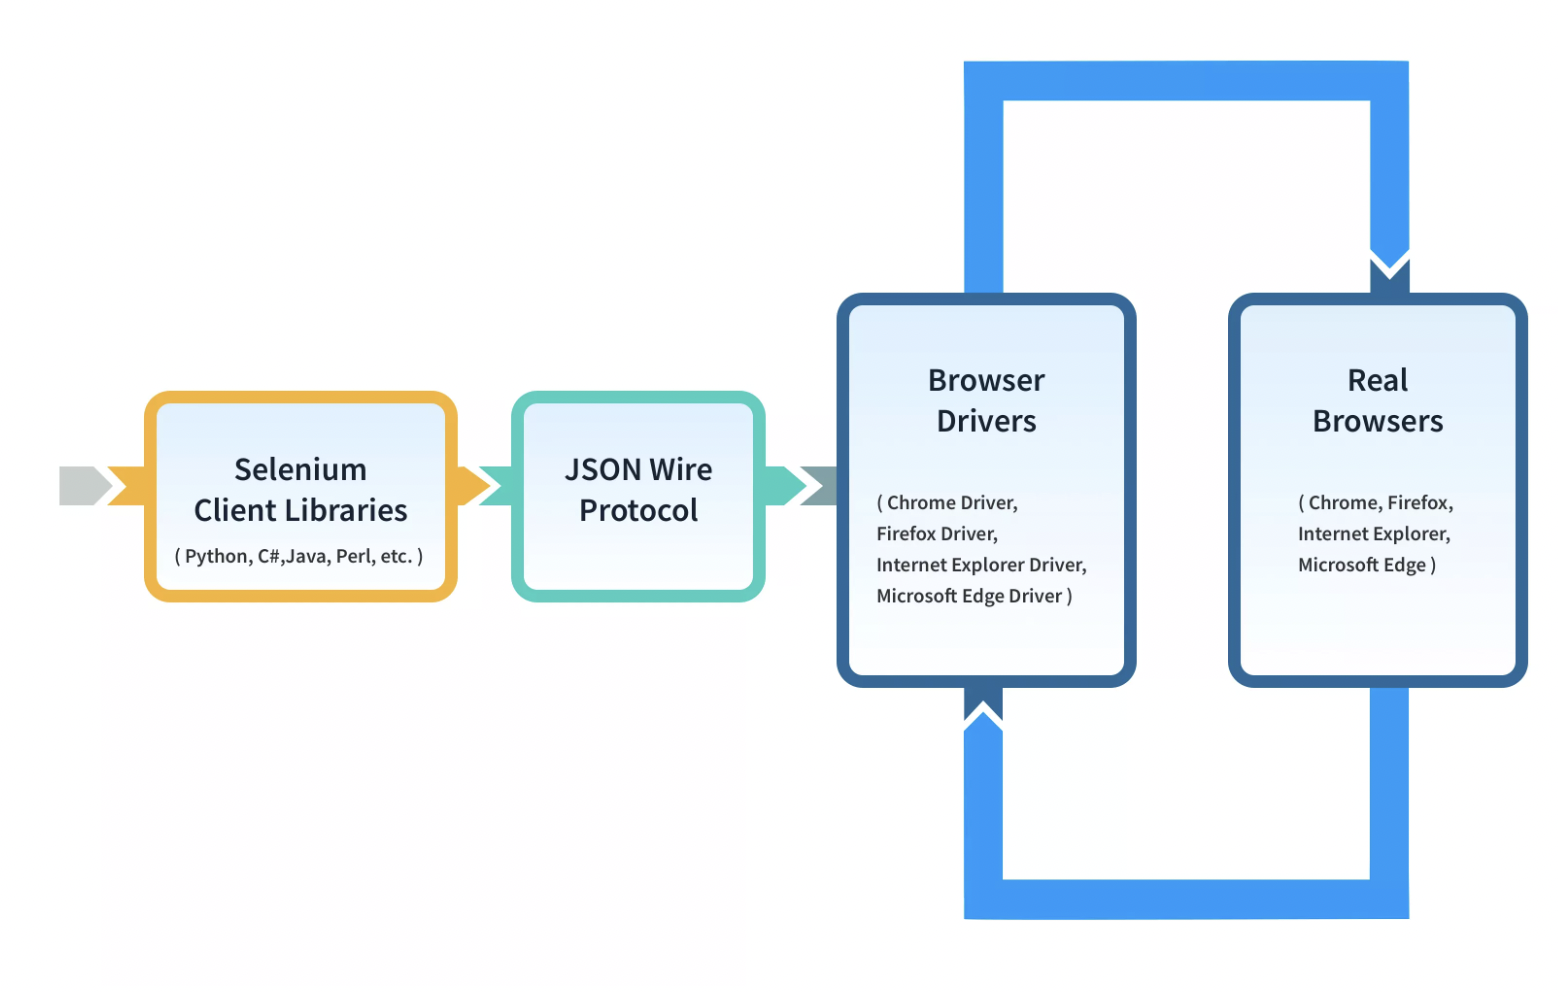
\includegraphics[width=0.9\textwidth]{imagenes/02-marco-teorico/arquitectura-selenium.png}
  \caption[Arquitectura de Selenium]{Arquitectura de Selenium \cite{selenium_webdriver}.}
  \label{fig:selenium}
\end{figure}

\subsubsection{Beautiful Soup}

Beautiful Soup es una biblioteca de Python utilizada para extraer datos de
archivos HTML y XML. Funciona junto con tu analizador de sintaxis preferido,
ofreciendo maneras idiomáticas de navegar, buscar y modificar el árbol de análisis.
Esta biblioteca suele ahorrar a los programadores horas o días de trabajo \cite{beautiful_soup}.

Esta librería se caracteriza por enfocarse en la extracción de datos de archivos
cuyo contenido sea estático y por lo tanto no se recomienda su uso en páginas
cuyo contenido sea dinámico \cite{beautiful_soup}. La web hoy en día está
compuesta en su gran mayoría por páginas dinámicas, por lo que el uso de esta
librería no es recomendable si se desea extraer información de este tipo
de páginas.

\subsubsection{Scrapy}

Scrapy es un marco de aplicación para rastrear sitios web y extraer datos
estructurados que pueden ser utilizados en una amplia gama de aplicaciones útiles,
como minería de datos, procesamiento de información o archivo histórico. Aunque
originalmente se diseñó para el web scraping, también es útil para extraer datos
mediante APIs o como un \textit{web scraper} de propósito general \cite{scrapy_overview}.

\subsubsection{cURL}

cURL es un proyecto enfocado en dos productos principales: curl, una herramienta
de línea de comandos, y libcurl, una biblioteca de transferencia con una API en C.
Ambos productos realizan transferencias en Internet de recursos especificados
como URLs mediante protocolos de Internet. cURL se dedica a todo lo relacionado
con las transferencias de protocolos de Internet, evitando manejar los datos
transferidos en sí. Por ejemplo, carece de conocimiento sobre HTML, pero domina
cómo transferir esos datos a través de HTTP. Estos productos se utilizan no solo
en una multitud de scripts y aplicaciones conectadas a Internet, sino también
en pruebas de servidores y experimentación con protocolos, estando presentes
en una variedad de dispositivos integrados donde se requieren transferencias
por Internet \cite{curl_project}.

A pesar de que cURL no es necesariamente una herramienta de \textit{web scraping},
es una herramienta que permite realizar peticiones HTTP de forma clara y
transparente, por lo que puede ser utilizada para realizar \textit{web scraping}
en situaciones dónde se requieren emular comportamientos de usuarios de forma
más avanzada que con otras herramientas de \textit{web scraping}.

\subsection{Archivos CSV}

Un archivo \acrlong{csv} es un archivo de texto que contiene valores separados por comas.
Estos archivos se utilizan para el intercambio de datos entre diferentes
aplicaciones. Por ejemplo, bases de datos y hojas de cálculo. Los archivos CSV
contienen datos tabulares, es decir, datos presentados en columnas separadas
por un carácter separador (generalmente una coma, pero a veces un punto y coma
o una pestaña) y filas (líneas). Cada fila debe contener la misma cantidad de
campos \cite{shafranovich2005common}.

El formato de valores separados por comas (CSV) se ha utilizado para intercambiar
y convertir datos entre varios programas de hojas de cálculo durante bastante tiempo.
Aunque este formato es muy común, nunca ha sido documentado formalmente. Además,
a pesar de que el árbol de registro MIME de IANA incluye un registro para el tipo
"text/tab-separated-values", nunca se han registrado tipos MIME para CSV con IANA.
Diferentes programas y sistemas operativos han comenzado a usar diferentes tipos
MIME para este formato. Este RFC documenta el formato de los archivos CSV y
registra formalmente el tipo MIME "text/csv" para CSV de acuerdo con el RFC 2048
\cite{shafranovich2005common}.


Aunque existen varias especificaciones e implementaciones para el formato CSV,
no existe una especificación formal, lo que permite una amplia variedad de
interpretaciones de los archivos CSV. Esta sección documenta el formato que
parece ser seguido por la mayoría de las implementaciones:

\begin{enumerate}
    \item Cada registro se ubica en una línea separada, delimitada por un salto
      de línea (CRLF). Por ejemplo:

    aaa,bbb,ccc CRLF \\
    zzz,yyy,xxx CRLF

    \item El último registro en el archivo puede o no tener un salto de línea
      final. Por ejemplo:

    aaa,bbb,ccc CRLF \\
    zzz,yyy,xxx

    \item Puede haber una línea de encabezado opcional que aparece como la
      primera línea del archivo con el mismo formato que las líneas de registro
      normales. Este encabezado contendrá nombres correspondientes a los campos
      en el archivo y debe contener el mismo número de campos que los registros
      en el resto del archivo (la presencia o ausencia de la línea de encabezado
      debe indicarse mediante el parámetro opcional "header" de este tipo MIME).
      Por ejemplo:

    field\_name,field\_name,field\_name CRLF \\
    aaa,bbb,ccc CRLF \\
    zzz,yyy,xxx CRLF
\end{enumerate}

Debido a la naturaleza del proyecto, los archivos CSV juegan un papel fundamental
en el almacenamiento de los datos obtenidos mediante \textit{web scraping}. Y
serán referidos en múltiples puntos del mismo para detallar su estructura y
contenido.

\section{Servicios Web}
Internet representa una red global que interconecta una inmensa cantidad de
computadoras de distintos tipos y redes. Los servicios web en la World Wide Web
actúan como métodos estandarizados para facilitar la comunicación entre aplicaciones
cliente y servidor. Estos servicios son módulos de software diseñados para
realizar funciones específicas y son accesibles en la computación en la nube a
través de la red. Su principal función es proporcionar capacidades específicas
a los clientes que los solicitan \cite{Wikipedia_Web_Service}.

Los servicios web se definen como un conjunto de protocolos y estándares abiertos
que posibilitan el intercambio de datos entre diferentes aplicaciones o sistemas.
Son fundamentales para permitir la interacción entre programas escritos en
diversos lenguajes de programación y ejecutados en múltiples plataformas, facilitando
así la transferencia de datos a través de redes como Internet. Estos servicios
utilizan protocolos web estandarizados, principalmente HTTP o HTTPS, y a menudo
intercambian información en formato XML o JSON, lo que permite una interacción fluida y
eficaz entre clientes y servidores a través de la red \cite{GeeksforGeeks_Web_Services}.

En la Figura \ref{fig:web-service} se muestra un diagrama general de arquitectura
de un servicio web.

\begin{figure}[!htbp]
  \centering
  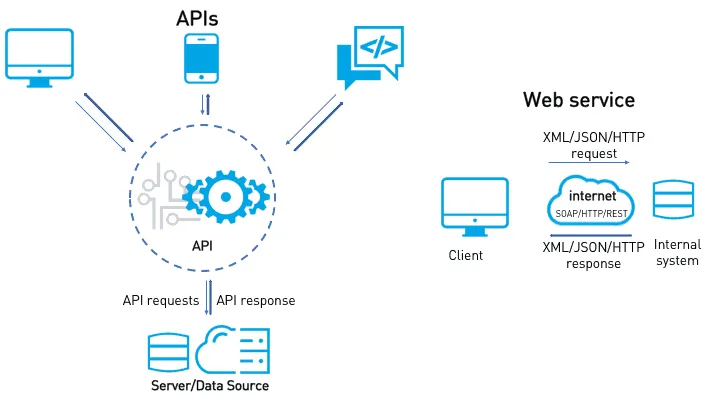
\includegraphics[width=0.9\textwidth]{imagenes/02-marco-teorico/arquitectura-servicio-web.png}
  \caption[Arquitectura de un Servicio Web]{Arquitectura de un Servicio Web \cite{beltran2023servicioweb}.}
  \label{fig:web-service}
\end{figure}

\subsection{Python}
Python es un lenguaje de programación de alto nivel, interpretado y orientado a
objetos, que se caracteriza por su dinamismo semántico. Sus estructuras de datos
integradas de alto nivel, junto con la tipificación y vinculación dinámicas, lo
hacen especialmente atractivo para el Desarrollo Rápido de Aplicaciones, así
como para ser utilizado como lenguaje de script o de ``pegamento'' para integrar
componentes ya existentes. La sintaxis de Python es sencilla y fácil de aprender,
lo que destaca su legibilidad y reduce así el costo del mantenimiento de programas.
Python apoya el uso de módulos y paquetes, fomentando la modularidad de los
programas y la reutilización de código. El intérprete de Python y su amplia
biblioteca estándar están disponibles de forma gratuita, tanto en código fuente
como en forma binaria, para todas las plataformas principales y pueden distribuirse
libremente \cite{Python_org}.

\begin{figure}[!htbp]
  \centering
  
\includegraphics[width=0.2\textwidth]{imagenes/02-marco-teorico/logo-python.png}
  \caption[Logo de Python]{Logo de Python \cite{Python_org}.}
  \label{fig:python-logo}
\end{figure}

\subsubsection{Usos de Python}

\begin{itemize}
  \item Desarrollo web (lado del servidor)
  \item Desarrollo de software
  \item Matemáticas
  \item Scripting de sistemas
\end{itemize}

\subsubsection{¿Qué puede hacer Python?}
\begin{itemize}
  \item Puede usarse en un servidor para crear aplicaciones web.
  \item Puede emplearse junto con software para crear flujos de trabajo.
  \item Puede conectarse a sistemas de bases de datos y leer y modificar archivos.
  \item Es útil para manejar grandes volúmenes de datos y realizar matemáticas complejas.
  \item Sirve tanto para prototipos rápidos como para el desarrollo de software listo para producción.
\end{itemize}

\subsubsection{¿Por qué Python?}
\begin{itemize}
  \item Funciona en diferentes plataformas (Windows, Mac, Linux, Raspberry Pi, etc.).
  \item Tiene una sintaxis simple similar al idioma inglés.
  \item La sintaxis de Python permite a los desarrolladores escribir programas con menos líneas que en otros lenguajes de programación.
  \item Es un lenguaje interpretado, lo que permite ejecutar el código tan pronto como se escribe, facilitando un prototipado rápido.
  \item Puede tratarse de manera procedural, orientada a objetos o funcional.
\end{itemize}

\subsubsection{Sintaxis de Python comparada con otros lenguajes de programación}
\begin{itemize}
  \item Fue diseñado para ser legible, con similitudes al idioma inglés y con influencia de las matemáticas.
  \item Utiliza nuevas líneas para completar un comando, a diferencia de otros lenguajes de programación que a menudo usan punto y coma o paréntesis.
  \item Se basa en la indentación, utilizando espacios en blanco, para definir el ámbito, como en bucles, funciones y clases. Otros lenguajes de programación a menudo usan llaves para este propósito.
\end{itemize}

Algunos de los \textit{frameworks} más utilizados para el desarrollo web con Python
son Django, Flask y FastAPI. A continuación se abordará cada uno de ellos.

\subsubsection{Flask}

Flask es un marco de trabajo (\textit{framework}) web escrito en Python, conocido por
ser un módulo que facilita el desarrollo de aplicaciones web. Se caracteriza por
tener un núcleo pequeño y fácil de ampliar, clasificándose como un microframework.
A diferencia de otros frameworks, Flask no incluye un ORM (Object Relational Manager)
ni características similares \cite{Flask_Documentation}.

\begin{figure}[!htbp]
  \centering
  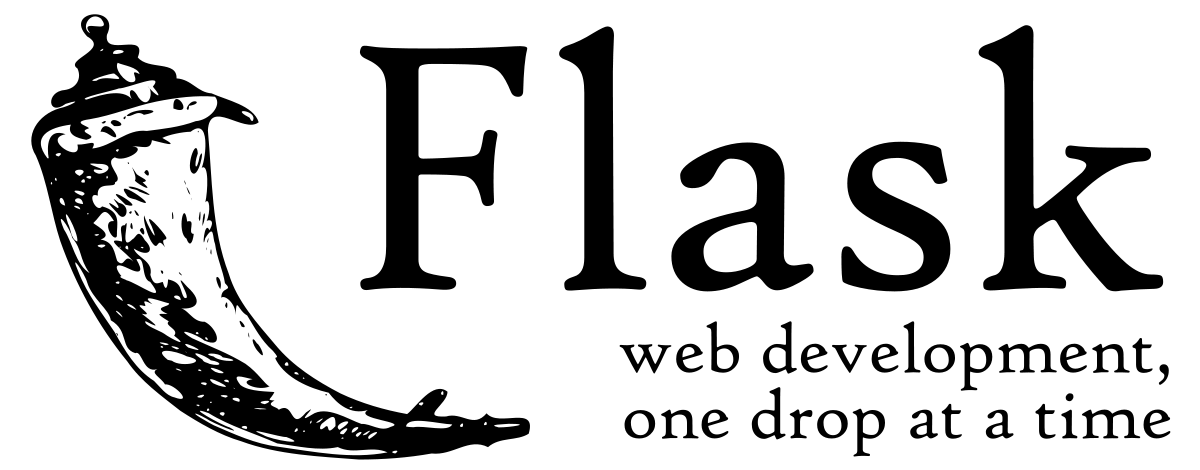
\includegraphics[width=0.6\textwidth]{imagenes/02-marco-teorico/logo-flask.png}
  \caption[Logo de Flask]{Logo de Flask \cite{Flask_Documentation}.}
  \label{fig:flask-logo}
\end{figure}

Entre sus características destacadas se encuentran la capacidad de enrutamiento
de URL y un motor de plantillas. Flask se basa en el conjunto de herramientas WSGI
(Web Server Gateway Interface) de Werkzeug y en el motor de plantillas Jinja2,
ambos proyectos de Pocco \cite{Python_Basics_Flask}.

Un marco de trabajo web es una colección de bibliotecas y módulos que permiten
a los desarrolladores de aplicaciones web escribir aplicaciones sin preocuparse
por detalles de bajo nivel como el protocolo o la gestión de hilos. WSGI, en
particular, es una especificación de interfaz común entre servidores web y
aplicaciones web. Werkzeug implementa objetos de solicitud y respuesta, y
funciones de utilidad, lo que permite la construcción de marcos web sobre él.
Jinja2 es un motor de plantillas que permite integrar variables de Python en
plantillas HTML \cite{Python_Basics_Flask}.

Flask se considera un microframework porque mantiene el núcleo de la aplicación
simple y escalable, permitiendo extensiones para agregar capacidades como
soporte de base de datos. A diferencia de Django, Flask es muy ``Pythonic'' y
tiene una curva de aprendizaje baja. Su simplicidad y explicitud aumentan la
legibilidad y permiten empezar proyectos rápidamente con pocas líneas de código.
Flask permite desarrollar tanto en un entorno
local como en línea, y es popular por ser actualizado, moderno y extensible,
permitiendo al desarrollador tomar decisiones sobre bases de datos, ORM, etc.
Flask es adecuado tanto para prototipos rápidos como para el desarrollo de
software listo para la producción y puede manejar aplicaciones complejas, a
pesar de su naturaleza de microframework \cite{Flask_Documentation}.

\subsubsection{Django}
Django es un framework web de Python de alto nivel diseñado para el desarrollo rápido de sitios web seguros y fáciles de mantener, destacándose por su comunidad activa, código abierto y amplias opciones de soporte \cite{MDN_Web_Docs_Django}.

\begin{figure}[!htbp]
  \centering
  
\includegraphics[width=0.4\textwidth]{imagenes/02-marco-teorico/logo-django.png}
  \caption[Logo de Django]{Logo de Django \cite{MDN_Web_Docs_Django}.}
  \label{fig:django-logo}
\end{figure}

Django se caracteriza por enfocarse en las siguientes características:

\begin{itemize}
  \item \textbf{Completo:} Ofrece una amplia gama de funcionalidades integradas para un desarrollo web eficiente y coherente.
  \item \textbf{Versátil:} Adecuado para construir una variedad de sitios web y compatible con múltiples formatos de entrega de contenido.
  \item \textbf{Seguro:} Incluye medidas de seguridad incorporadas para prevenir errores comunes y proteger la web.
  \item \textbf{Escalable:} Su arquitectura basada en componentes independientes permite un escalado eficaz para manejar más tráfico.
  \item \textbf{Mantenible:} Promueve la creación de código reutilizable y bien organizado, alineado con los principios de diseño limpio.
  \item \textbf{Portable:} Escrito en Python, funciona en varias plataformas y es compatible con numerosos proveedores de hosting.
\end{itemize}

\subsubsection{FastAPI}

FastAPI es un moderno y rápido framework de alto rendimiento para la creación
de APIs con Python 3.8 o superior, basado en las pistas de tipo estándar de Python.
Este framework se destaca por su alta performance y facilidad de uso, ofreciendo
una solución eficiente y escalable para el desarrollo de aplicaciones web y APIs
\cite{FastAPI_Official}.

\begin{figure}[!htbp]
  \centering
  
\includegraphics[width=0.4\textwidth]{imagenes/02-marco-teorico/fastapi-logo.png}
  \caption[Logo de FastAPI]{Logo de FastAPI \cite{FastAPI_Official}.}
  \label{fig:fastapi-logo}
\end{figure}

Las características más destacadas de FastAPI son:

\begin{itemize}
    \item \textbf{Rápido:} Ofrece un rendimiento muy alto, comparable con NodeJS
      y Go, gracias a Starlette y Pydantic, siendo uno de los frameworks de Python
      más rápidos disponibles.
    \item \textbf{Ágil para programar:} Permite aumentar la velocidad de desarrollo
      de características en aproximadamente un 200\% a 300\%.
    \item \textbf{Menos errores:} Reduce en un 40\% los errores inducidos por los
      desarrolladores.
    \item \textbf{Intuitivo:} Ofrece un gran soporte para editores de código, con
      completado automático en todas partes, lo que disminuye el tiempo dedicado
      a la depuración.
    \item \textbf{Fácil de usar:} Diseñado para ser fácil de aprender y utilizar,
      minimizando el tiempo necesario para leer documentación.
    \item \textbf{Conciso:} Minimiza la duplicación de código. Múltiples
      características a partir de cada declaración de parámetro, lo que conlleva
      a menos errores.
    \item \textbf{Robusto:} Genera código listo para producción, con documentación
      interactiva automática.
    \item \textbf{Basado en estándares:} Se basa en (y es completamente compatible
      con) los estándares abiertos para APIs: OpenAPI (anteriormente conocido
      como Swagger) y JSON Schema.
\end{itemize}

\subsection{API}

Una API (Interfaz de Programación de Aplicaciones) es un conjunto de definiciones
y protocolos para construir e integrar software de aplicaciones. Funciona
como un contrato entre un proveedor de información y un usuario, especificando
lo que se necesita tanto en la solicitud (llamada) como en la respuesta. Permite
la interacción con un sistema para obtener información o realizar funciones,
actuando como mediador entre los usuarios o clientes y los recursos o servicios
web que desean obtener. Las APIs son clave para compartir recursos e información
manteniendo la seguridad, el control y la autenticación, y simplifican la
interacción sin necesidad de conocer detalles específicos como el almacenamiento
en caché. \cite{Red_Hat_REST_API}.

\subsubsection{REST}
REST (Representational State Transfer) es un conjunto de restricciones
arquitectónicas, no un protocolo o estándar, que los desarrolladores de API
pueden implementar de diversas maneras. Cuando se realiza una solicitud a
través de una API REST, se transfiere una representación del estado del
recurso al solicitante o endpoint, en formatos como JSON, HTML, XLT, Python,
PHP o texto plano, siendo JSON el más popular por su agnosticismo de lenguaje
y legibilidad tanto para humanos como para máquinas \cite{Red_Hat_REST_API}. En
la Figura \ref{fig:rest-api} se muestra un diagrama general de arquitectura
de una API REST.

\begin{figure}[!htbp]
  \centering
  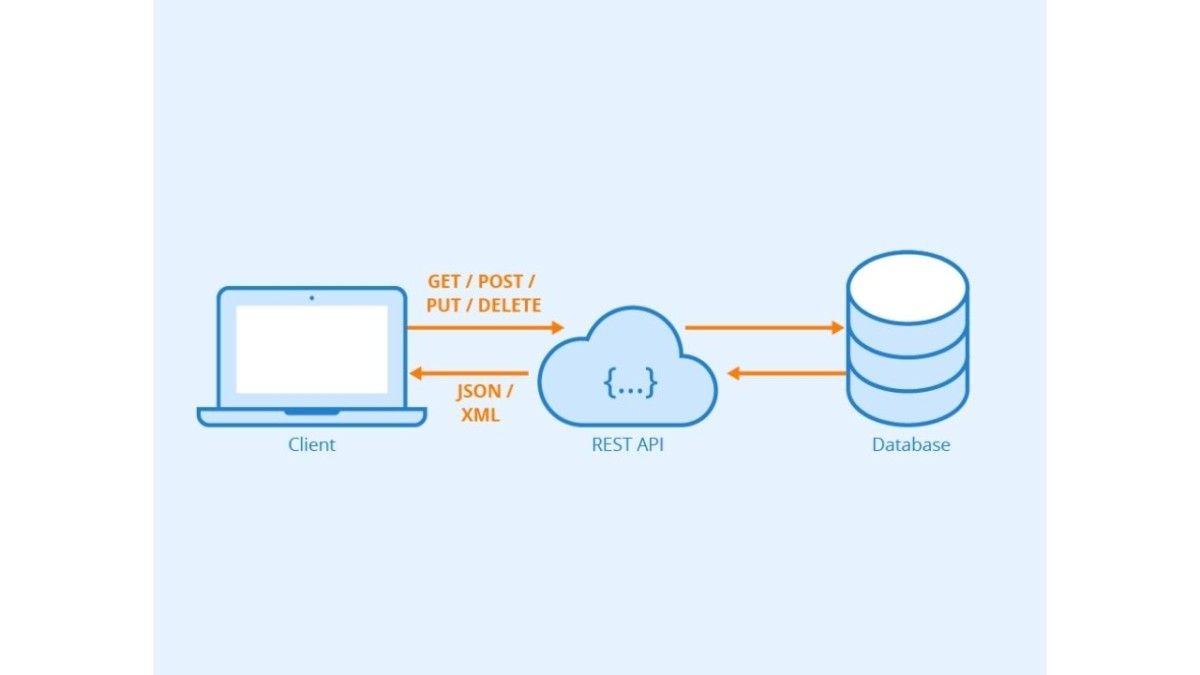
\includegraphics[width=0.9\textwidth]{imagenes/02-marco-teorico/rest-api-diagram.jpg}
  \caption[Arquitectura de una API REST]{Arquitectura de una API REST \cite{restapi_ironio}.}
  \label{fig:rest-api}
\end{figure}

Para que una API sea considerada RESTful, debe cumplir con ciertos criterios:
una arquitectura cliente-servidor con comunicación sin estado, datos cacheables,
una interfaz uniforme para la transferencia estándar de información, y un sistema
en capas. Incluye detalles como headers y parámetros en los métodos HTTP,
importantes para la metadata y autorización. A pesar de sus criterios específicos,
REST es más fácil de usar y flexible que protocolos como SOAP, lo que la hace
más rápida, ligera y escalable, ideal para el desarrollo de aplicaciones móviles
e Internet de las Cosas (IoT) \cite{Red_Hat_REST_API}.

\subsection{JSON}
\textit{JavaScript Object Notation (JSON)} es un formato estándar basado en texto
para representar datos estructurados basados en la sintaxis de objetos de JavaScript.
Se utiliza comúnmente para la transmisión de datos en aplicaciones web, tanto del
servidor al cliente como viceversa. JSON es un formato de datos basado en texto
que sigue la sintaxis de objeto de JavaScript, popularizado por Douglas Crockford.
Aunque se parece a la sintaxis literal de objeto de JavaScript, puede
usarse de manera independiente y es compatible con muchos entornos de
programación. JSON existe como una cadena de texto y necesita convertirse a
un objeto JavaScript nativo para acceder a los datos. Esta conversión se conoce
como deserialización, mientras que convertir un objeto nativo a una cadena para
su transmisión se llama serialización. Una cadena JSON puede almacenarse en un
archivo propio, con extensión \texttt{.json} y tipo MIME de \texttt{application/json}
\cite{MDN_Web_Docs_JSON}.

\subsection{SSL}
SSL (\textit{Secure Sockets Layer}) es una tecnología de encriptación desarrollada
originalmente por Netscape en la década de 1990. SSL establece una conexión
encriptada entre el servidor web y el navegador del visitante, permitiendo la
transmisión segura de información privada y protegiéndola contra la interceptación,
manipulación de datos y falsificación de mensajes. Para habilitar SSL en un sitio
web, se requiere obtener e instalar un Certificado SSL en el servidor web. Este
certificado puede ser identificado en los navegadores, a menudo mediante un icono
de candado o una barra de direcciones verde. La activación de SSL se realiza
cambiando el URL de \texttt{http://} a \texttt{https://}, asegurando la
encriptación de la información transmitida. Los Certificados SSL son emitidos
por Autoridades Certificadoras (CAs) y son ampliamente utilizados por negocios
en línea para proteger sus sitios web y generar confianza en sus clientes
\cite{SSL_Shopper_SSL}.

\subsection{HTTPS}

HTTPS (\textit{Hypertext Transfer Protocol Secure}) es la versión segura de HTTP,
el protocolo principal para enviar datos entre un navegador web y un sitio web.
HTTPS encripta los datos para aumentar la seguridad en la transferencia, lo cual
es crucial cuando los usuarios transmiten información sensible, como al iniciar
sesión en cuentas bancarias, servicios de correo electrónico o proveedores de
seguros de salud. Los sitios web, en especial aquellos que requieren credenciales
de inicio de sesión, deben utilizar HTTPS. Los navegadores modernos, como Chrome,
marcan los sitios que no utilizan HTTPS como no seguros. Un candado en la barra
de URL indica que la página web es segura \cite{Cloudflare_HTTPS}.

\subsection{DNS}
DNS (\textit{Domain Name System}) es un sistema que traduce el nombre de una
máquina en red (host) a una dirección IP legible por máquina, asegurando que
los paquetes se enrutan correctamente en la red. Por razones de seguridad, un
servidor en la red puede usar una ``búsqueda inversa'' para confirmar a sus
administradores que las personas adecuadas se están conectando a él. Algunos
servidores web o ftp no permiten conexiones a menos que puedan mapear inversamente
la dirección IP a un nombre de host registrado \cite{cornell_dns}.

\subsection{CDN}
Un CDN (\textit{Content Delivery Network}) es un conjunto de servidores
distribuidos en múltiples ubicaciones. Estos servidores almacenan copias
duplicadas de datos para responder a solicitudes basándose en cuáles están más
cerca de los usuarios finales, lo que resulta en un servicio rápido y menos
afectado por alto tráfico. Los CDNs son ampliamente utilizados para entregar
hojas de estilo y archivos JavaScript (activos estáticos) de bibliotecas como
Bootstrap, jQuery, etc. Usar un CDN para estos archivos es preferible por varias
razones: reduce la carga de solicitudes en los servidores propios de una
organización, los servidores de CDN pueden estar geográficamente más cerca de
los usuarios, y los CDN ya están configurados con ajustes de caché adecuados,
lo que ahorra configuración adicional en los propios servidores \cite{mdn_cdn}.

\subsection{Docker}

Docker es una plataforma abierta para desarrollar, distribuir y ejecutar
aplicaciones, permitiendo separar las aplicaciones de la infraestructura para
agilizar la entrega de software. Con Docker, se puede gestionar la infraestructura
de la misma manera que las aplicaciones, aprovechando sus metodologías para
distribuir, probar y desplegar código, reduciendo así el tiempo entre la escritura
del código y su ejecución en producción \cite{docker_overview}.

\subsubsection{La plataforma Docker}
Docker posibilita empaquetar y ejecutar aplicaciones en un entorno aislado
llamado contenedor, que es seguro y permite la ejecución simultánea de múltiples
contenedores en un mismo host. Los contenedores son ligeros y contienen todo lo
necesario para ejecutar la aplicación, lo que elimina la dependencia del software
instalado en el host \cite{docker_overview}. Docker también proporciona herramientas y una plataforma
para gestionar el ciclo de vida de los contenedores, lo que incluye:

\begin{itemize}
    \item Desarrollar la aplicación y sus componentes de soporte usando contenedores.
    \item El contenedor se convierte en la unidad para distribuir y probar la aplicación.
    \item Al estar listo, desplegar la aplicación en el entorno de producción,
      ya sea como un contenedor o un servicio orquestado, funcionando igual en
      un centro de datos local, un proveedor de nube o una combinación de ambos.
\end{itemize}

En la Figura \ref{fig:docker} se muestra un diagrama general de arquitectura
de Docker.

\begin{figure}[!htbp]
  \centering
  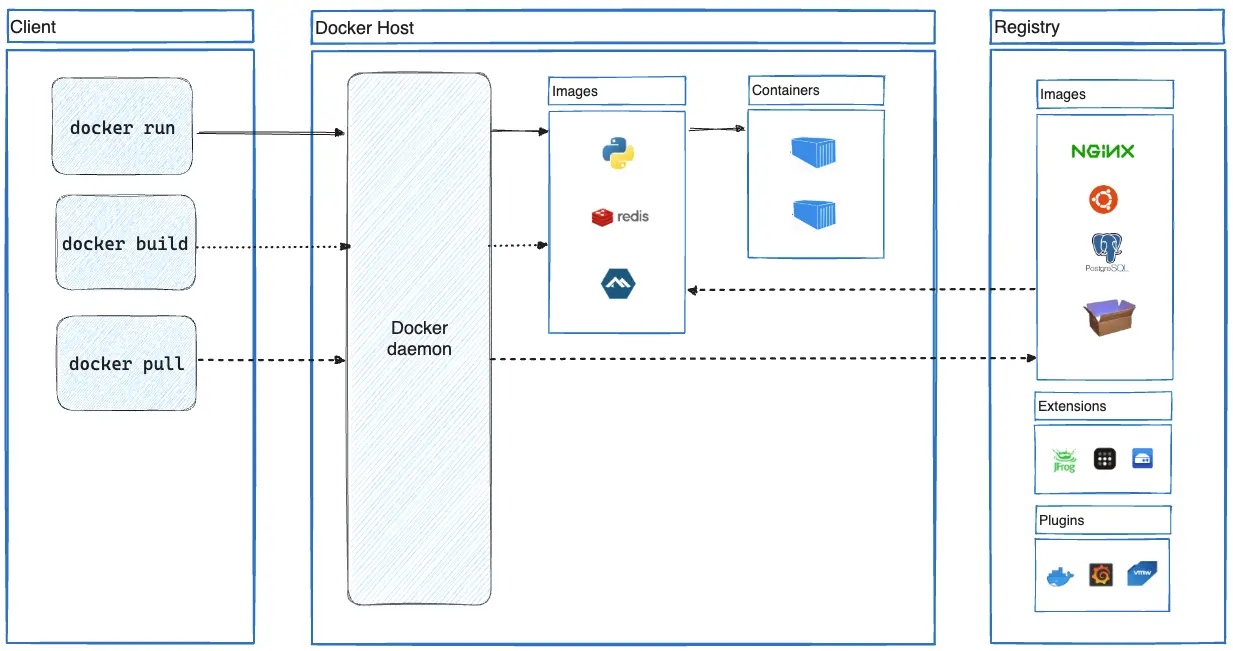
\includegraphics[width=0.9\textwidth]{imagenes/02-marco-teorico/arquitectura-docker.png}
  \caption[Arquitectura de Docker]{Arquitectura de Docker \cite{docker_overview}.}
  \label{fig:docker}
\end{figure}


\section{Aplicación Web}
Una aplicación web es una aplicación invocada a través de un navegador web en
Internet. Desde su auge en la década de 1990, la web ha evolucionado de ser un
repositorio de páginas estáticas a una poderosa plataforma para el desarrollo y
despliegue de aplicaciones innovadoras. Las aplicaciones web actuales permiten
una nueva modalidad de cooperación y colaboración entre usuarios, soportando
tanto datos estructurados como no estructurados, y ofreciendo interfaces de
navegación exploratorias. Las aplicaciones web modernas, dentro del concepto de
Web 2.0, son dinámicas e invitan a la participación del usuario, siendo más
responsivas y cercanas a las aplicaciones de escritorio. El desarrollo de
aplicaciones web ha adoptado técnicas de ingeniería de software como la
orientación a servicios, y sigue evolucionando rápidamente, anticipando nuevas
tendencias y enfoques en el futuro \cite{4221621}.

\subsection{JavaScript}
JavaScript (JS) es un lenguaje de programación ligero e interpretado (o compilado
justo a tiempo) con funciones de primera clase. Aunque es más conocido como el
lenguaje de scripting para páginas web, también se utiliza en entornos fuera del
navegador, como Node.js, Apache CouchDB y Adobe Acrobat. JS es un lenguaje
basado en prototipos, de paradigma múltiple, de un solo hilo y dinámico, que
admite estilos de programación orientada a objetos, imperativa y declarativa.
Las capacidades dinámicas de JavaScript incluyen la construcción de objetos en
tiempo de ejecución, listas de parámetros variables, variables de función,
creación dinámica de scripts (a través de \texttt{eval}), introspección de objetos
y recuperación del código fuente. Este lenguaje se rige por los estándares
ECMAScript (ECMA-262) y la API de Internacionalización ECMAScript (ECMA-402).
Es importante no confundir JavaScript con el lenguaje de programación Java, ya
que, a pesar de sus nombres similares, tienen sintaxis, semánticas y usos muy
diferentes \cite{mdn_javascript}.

\begin{figure}[!htbp]
  \centering
  
\includegraphics[width=0.2\textwidth]{imagenes/02-marco-teorico/javascript-logo.png}
  \caption[Logo de JavaScript]{Logo de JavaScript \cite{mdn_javascript}.}
  \label{fig:javascript-logo}
\end{figure}

\subsection{HTML}
HTML, o \textit{Hypertext Markup Language}, es el lenguaje de marcado estándar
utilizado para crear páginas web. Es uno de los pilares fundamentales de la
World Wide Web y es utilizado para estructurar el contenido y presentarlo en
Internet. HTML describe la estructura de una página web semánticamente y,
originalmente, incluía señales para la apariencia del documento \cite{whatwg_html_standard}.

\begin{figure}[!htbp]
  \centering
  
\includegraphics[width=0.2\textwidth]{imagenes/02-marco-teorico/html-logo.png}
  \caption[Logo de HTML]{Logo de HTML \cite{whatwg_html_standard}.}
  \label{fig:html-logo}
\end{figure}

HTML se compone de una serie de elementos que se utilizan para encerrar o envolver
diferentes partes del contenido para hacerlo actuar de cierta manera, o para
mostrarlo de cierta manera. Estos elementos están representados por etiquetas,
escritas con corchetes angulares. Por ejemplo, \texttt{<p>} representa un párrafo.
Algunas etiquetas tienen pares de apertura y cierre que encierran el contenido,
mientras que otras, como \texttt{<img>}, son autocontenidas \cite{whatwg_html_standard}.

Con el tiempo, HTML ha evolucionado significativamente. La versión actual, HTML5,
introduce una gran cantidad de tecnología y API para facilitar la creación de
sitios web y aplicaciones web complejas y ricas. HTML5 está diseñado para ser
utilizado en conjunto con CSS y JavaScript, permitiendo a los desarrolladores
crear experiencias de usuario interactivas y atractivas en la web \cite{whatwg_html_standard}.

\subsection{CSS}
CSS, o \textit{Cascading Style Sheets}, es un lenguaje de diseño gráfico utilizado
para definir y crear la presentación de un documento estructurado escrito en
HTML o XML. CSS describe cómo se deben mostrar los elementos en la pantalla,
en papel, en el habla o en otras formas de medios. Es fundamental para la creación
de páginas web visualmente atractivas y profesionalmente estilizadas \cite{w3c_css_home}.

\begin{figure}[!htbp]
  \centering
  
\includegraphics[width=0.2\textwidth]{imagenes/02-marco-teorico/css-logo.png}
  \caption[Logo de CSS]{Logo de CSS \cite{w3c_css_home}.}
  \label{fig:css-logo}
\end{figure}

Además de definir estilos como fuentes, colores y espaciado, CSS permite una gran
flexibilidad y control en la disposición visual de los elementos en una página web.
Se pueden establecer estilos específicos para diferentes dispositivos y tamaños de
pantalla, lo que permite que los sitios web sean responsivos y adaptables. CSS
también mejora la accesibilidad del contenido web y reduce la complejidad del
código HTML al separar la estructura del contenido de su presentación visual \cite{w3c_css_home}.

A pesar de que CSS en sí mismo ofrece una flexibilidad significativa, los
\textit{frameworks} CSS permiten un desarrollo web más rápido y eficiente,
proporcionando una base sólida para el diseño de sitios web. Algunos de los
\textit{frameworks} CSS más utilizados son Bootstrap, Material UI y Tailwind.

\subsubsection{Bootstrap}
Bootstrap es un marco (\textit{framework}) de código abierto para desarrollo web
front-end, que utiliza HTML, CSS y JavaScript. Su propósito es facilitar el
diseño de sitios y aplicaciones web responsivas y móviles. Bootstrap proporciona
una amplia gama de herramientas reutilizables como sistemas de grillas,
componentes predefinidos y potentes plugins basados en JavaScript. Diseñado
inicialmente por Twitter, Bootstrap se ha convertido en una de las herramientas
más populares para el desarrollo web, gracias a su enfoque en el diseño adaptativo
y la compatibilidad entre navegadores \cite{bootstrap_official}. En la Figura
\ref{fig:bootstrap-demo} se muestra un ejemplo de un sitio web desarrollado con
Bootstrap.

\begin{figure}[!htbp]
  \centering
  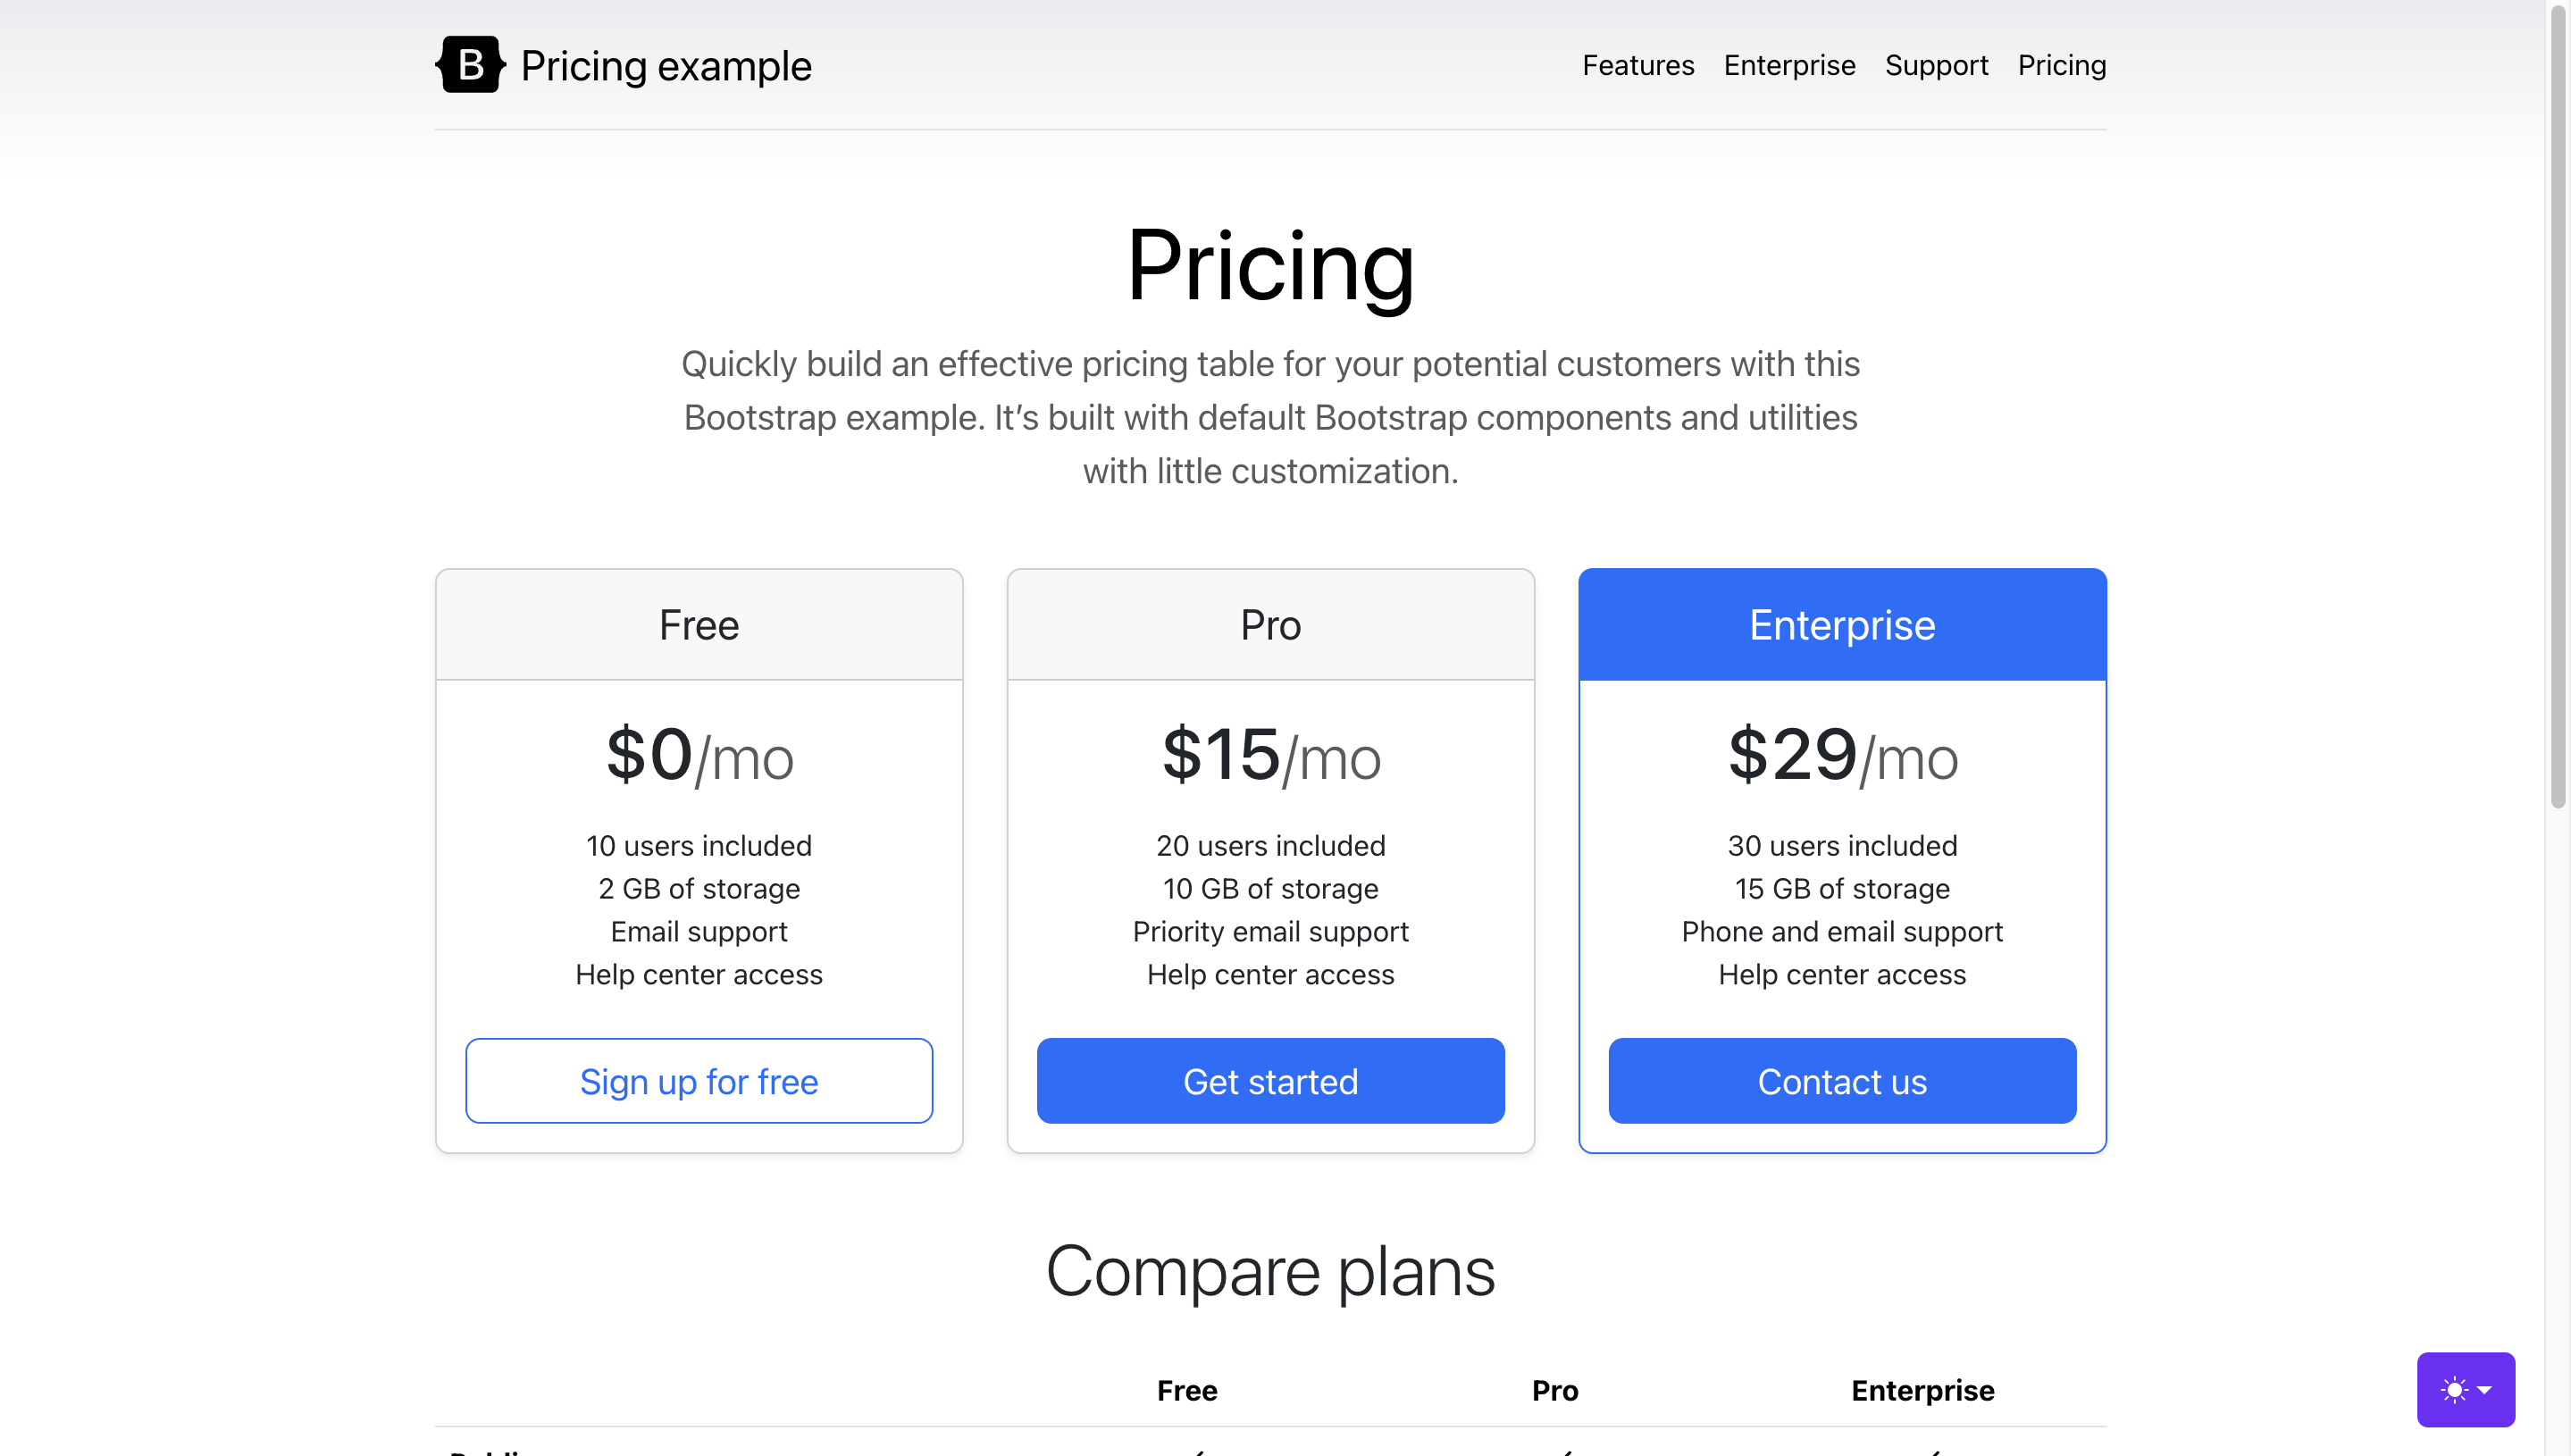
\includegraphics[width=0.9\textwidth]{imagenes/02-marco-teorico/bootstrap-demo.png}
  \caption[Ejemplo de sitio web desarrollado con Bootstrap]{Ejemplo de sitio web desarrollado con Bootstrap \cite{bootstrap_official}.}
  \label{fig:bootstrap-demo}
\end{figure}

\subsubsection{Material UI}
Material-UI es un \textit{framework} de interfaz de usuario para React que implementa
los principios de diseño de Material Design de Google. Proporciona un conjunto
de componentes de React reutilizables y personalizables que siguen las pautas de
Material Design, permitiendo desarrollar interfaces de usuario estéticamente
agradables y consistentes de manera eficiente. Material-UI es conocido por su
enfoque en la interactividad y la experiencia del usuario, ofreciendo una amplia
variedad de elementos de interfaz, desde simples botones y campos de texto hasta
componentes más complejos como diálogos y barras de navegación. Su diseño modular
y personalizable lo hace popular entre los desarrolladores de aplicaciones web
modernas \cite{mui_getting_started}. En la Figura \ref{fig:material-ui-demo} se
muestra un ejemplo de un sitio web desarrollado con Material-UI.

\begin{figure}[!htbp]
  \centering
  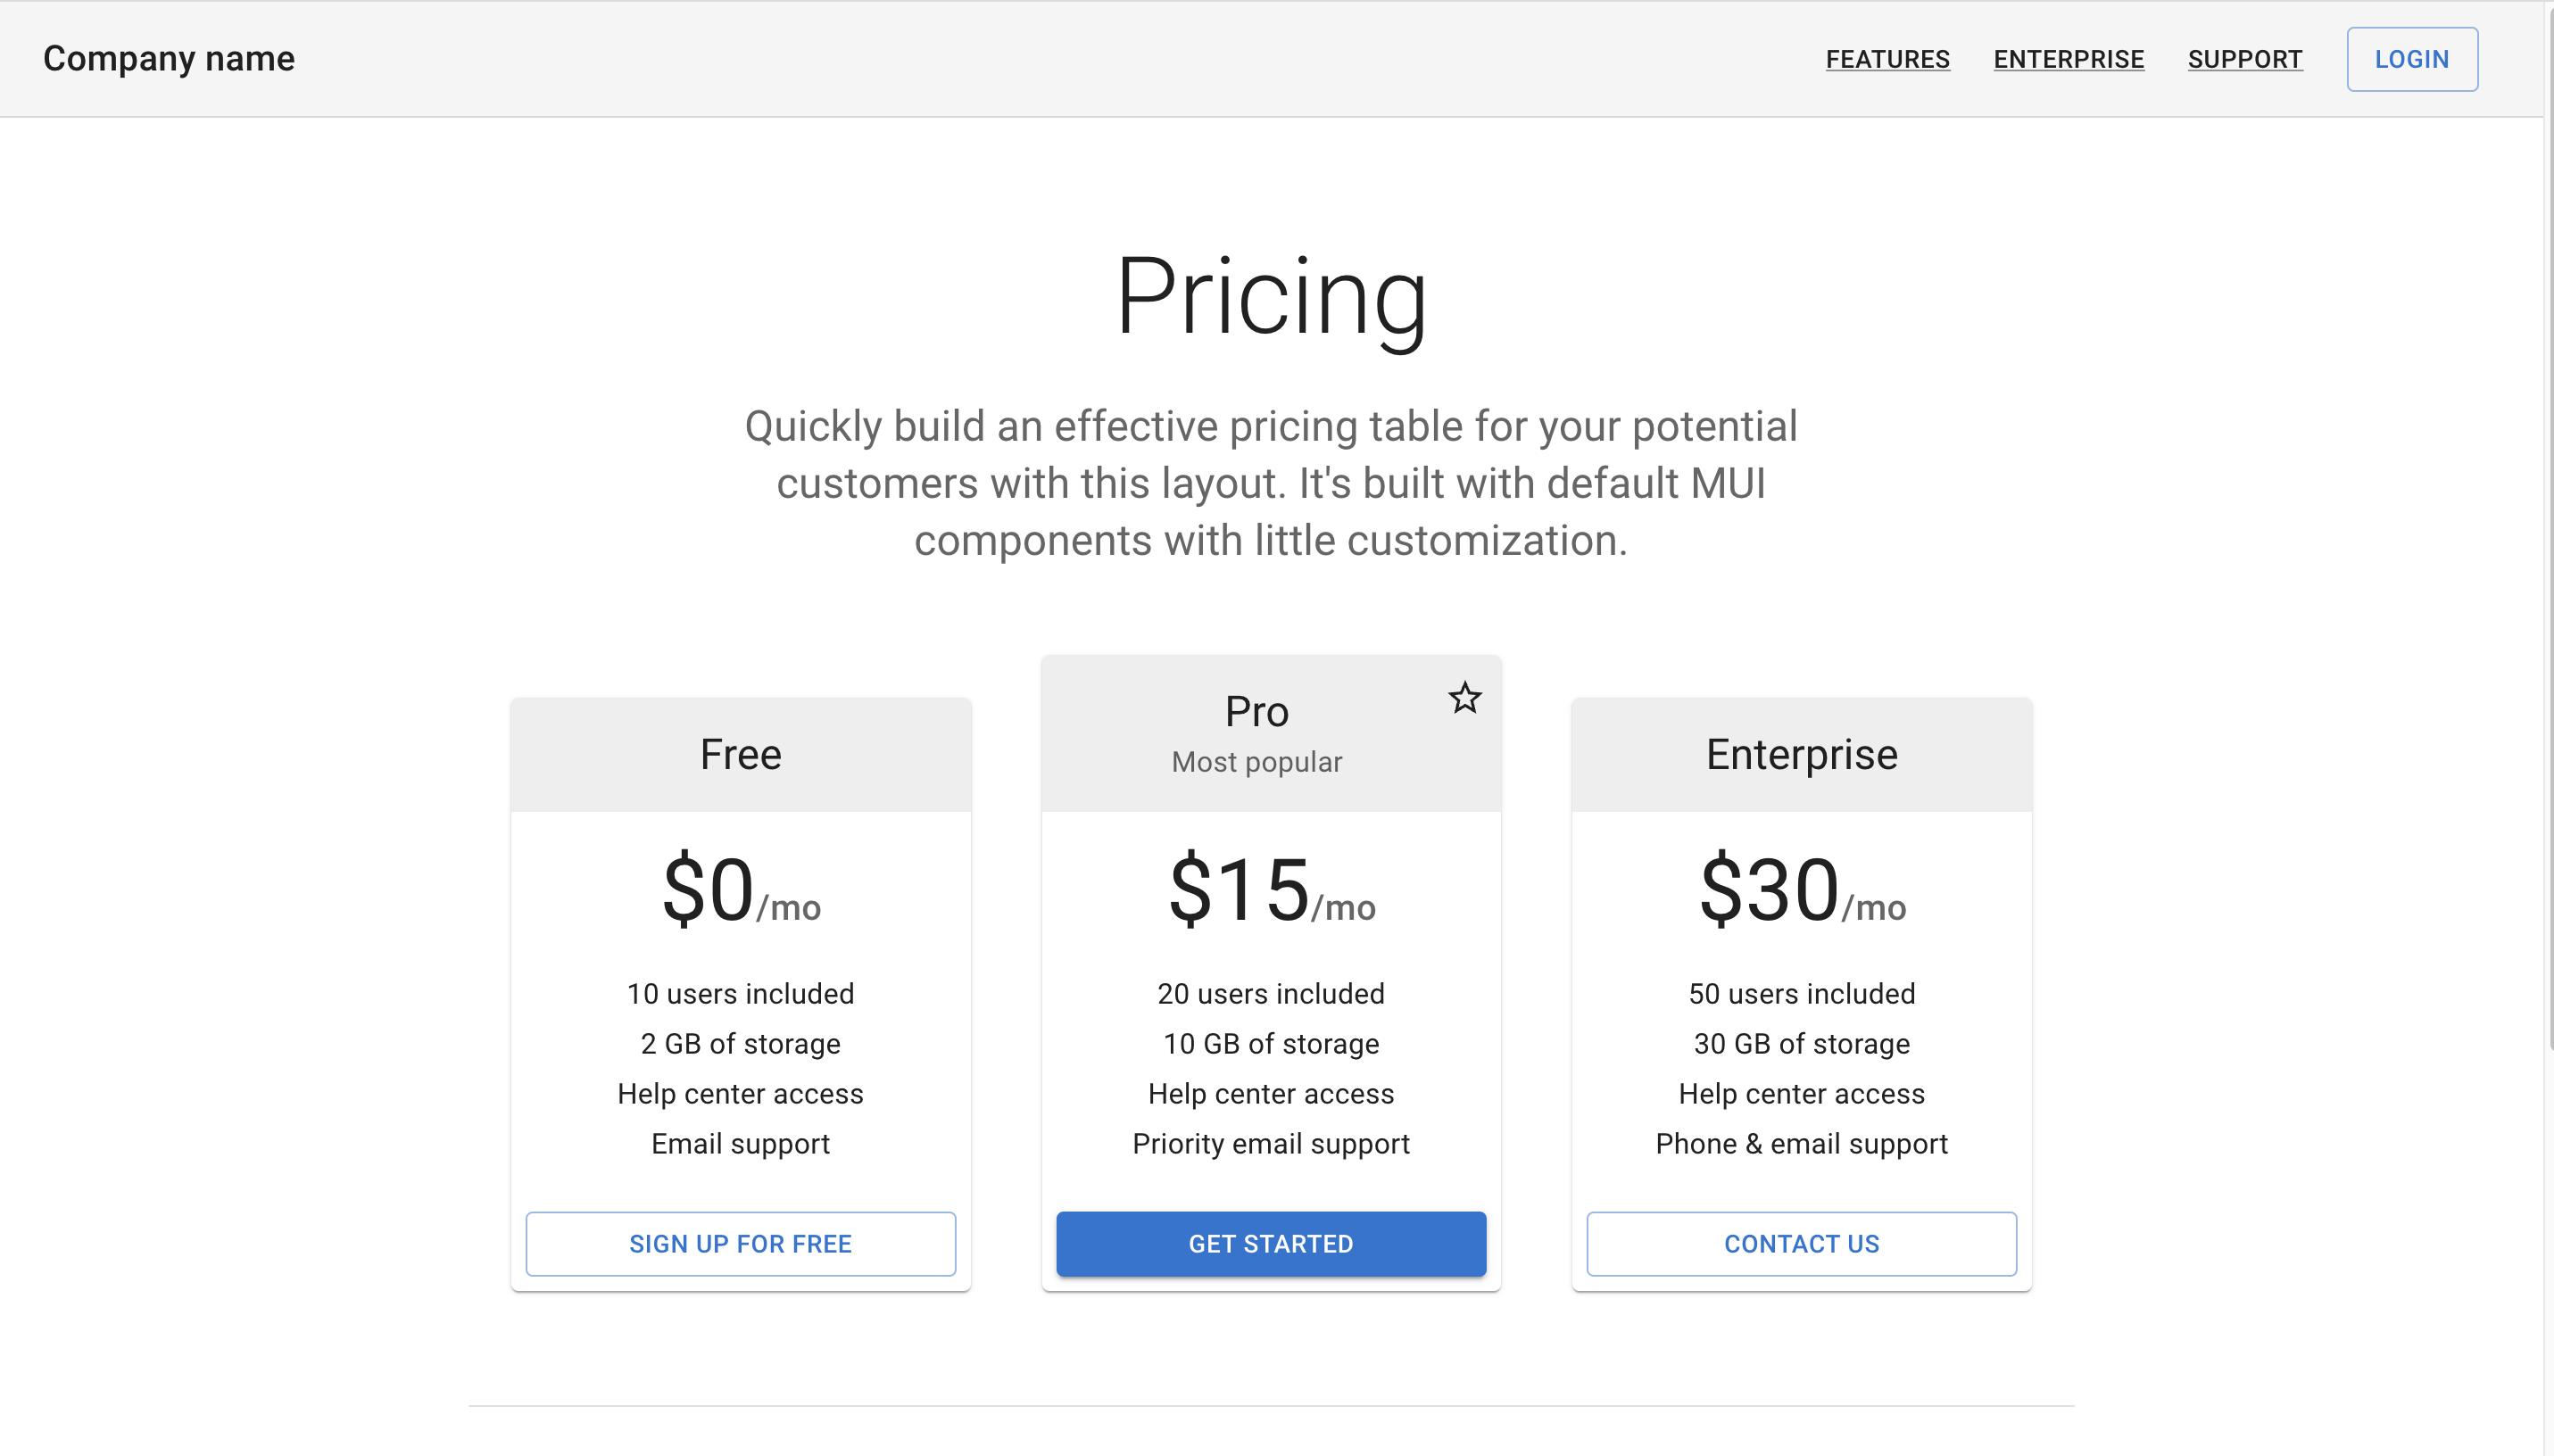
\includegraphics[width=0.9\textwidth]{imagenes/02-marco-teorico/material-ui-demo.png}
  \caption[Ejemplo de sitio web desarrollado con Material-UI]{Ejemplo de sitio web desarrollado con Material-UI \cite{mui_getting_started}.}
  \label{fig:material-ui-demo}
\end{figure}

\subsection{React}
React es una biblioteca de JavaScript para construir interfaces de usuario. Es
mantenido por Facebook y una comunidad de desarrolladores individuales y empresas.
React permite a los desarrolladores crear aplicaciones web grandes que pueden
cambiar datos, sin recargar la página. Su objetivo principal es ser rápido,
escalable y simple. Se puede usar con una combinación de otras bibliotecas o marcos
de JavaScript, como Angular JS en MVC \cite{ReactLearn2023}.

\begin{figure}[!htbp]
  \centering
  
\includegraphics[width=0.2\textwidth]{imagenes/02-marco-teorico/react-logo.png}
  \caption[Logo de React]{Logo de React \cite{ReactLearn2023}.}
  \label{fig:react-logo}
\end{figure}

Una característica clave de React es su enfoque en componentes. Los usuarios
definen componentes que manejan su propio estado, luego componen para formar
interfaces de usuario complejas. En lugar de trabajar con el modelo de objetos de
documento (DOM) del navegador, React crea un DOM virtual, donde se realizan sus
componentes y la lógica de estado. Esto proporciona un rendimiento mejorado, ya
que los cambios en el DOM virtual tienen menos costo de rendimiento que los
cambios en el DOM real. Además, React utiliza un enfoque declarativo que facilita
el razonamiento sobre el flujo de datos y la interfaz de usuario \cite{ReactLearn2023}.

\subsection{Vue}
Vue.js es un marco de JavaScript progresivo utilizado para construir interfaces
de usuario y aplicaciones de una sola página. Es conocido por su simplicidad,
facilidad de integración y enfoque en la experiencia del desarrollador. Vue se
basa en HTML, CSS y JavaScript estándar, proporcionando un modelo de programación
declarativo y basado en componentes que facilita el desarrollo de interfaces de
usuario, ya sean simples o complejas \cite{VuejsGuide2023}.

\begin{figure}[!htbp]
  \centering
  
\includegraphics[width=0.2\textwidth]{imagenes/02-marco-teorico/vue-logo.png}
  \caption[Logo de Vue]{Logo de Vue \cite{VuejsGuide2023}.}
  \label{fig:vue-logo}
\end{figure}

Una de las características clave de Vue es su sistema de reactividad, que rastrea
automáticamente los cambios en el estado del JavaScript y actualiza el DOM de
manera eficiente cuando estos cambios ocurren. Además, Vue es flexible y
adaptable, lo que permite su uso de diferentes maneras según el caso de uso,
incluyendo la mejora de HTML estático, la incorporación como componentes web en
cualquier página, aplicaciones de una sola página, renderizado en el lado del
servidor, generación de sitios estáticos y más. Su enfoque progresivo significa
que puede ser tan simple o robusto como lo necesite el proyecto, adaptándose y
creciendo con las necesidades del desarrollador \cite{VuejsGuide2023}.

\section{Plataforma de nube}

La \textit{computación en la nube} se refiere a un servicio basado en suscripción
donde se pueden obtener \textit{espacio de almacenamiento en red} y \textit{recursos informáticos}.
Similar a cómo funciona un cliente de correo electrónico como Yahoo!, Gmail o
Hotmail, que administra todo el hardware y software necesario para soportar
una cuenta de correo electrónico personal, la computación en la nube funciona
de manera análoga, pero proporcionando acceso a una variedad más amplia de
información y recursos. Esta tecnología permite acceder a la información
\textit{desde cualquier lugar y en cualquier momento}, siempre que se tenga
acceso a Internet, eliminando la necesidad de estar en la misma ubicación física
que el hardware que almacena los datos. Existen diferentes tipos de nubes, como
la \textit{Nube Pública}, \textit{Nube Privada}, \textit{Nube Comunitaria} y
\textit{Nube Híbrida}, cada una adaptada a necesidades específicas. Las empresas
pueden adaptar su uso del espacio en la nube según cambien sus necesidades, lo
que es especialmente útil para pequeñas empresas que buscan soluciones económicas
y escalables para el almacenamiento de datos y recursos informáticos \cite{huth2011basics}.

Existen múltiples proveedores de servicios de nube, como Google Cloud Platform,
Microsoft Azure y Amazon Web Services, que ofrecen una variedad de servicios
para el desarrollo de aplicaciones web y móviles, incluyendo almacenamiento,
bases de datos, redes, análisis, aprendizaje automático e inteligencia artificial,
entre otros. En la Figura \ref{fig:cloud-providers-market-share} se muestra la
distribución del mercado de proveedores de servicios de nube en el año 2023.

\begin{figure}[!htbp]
  \centering
  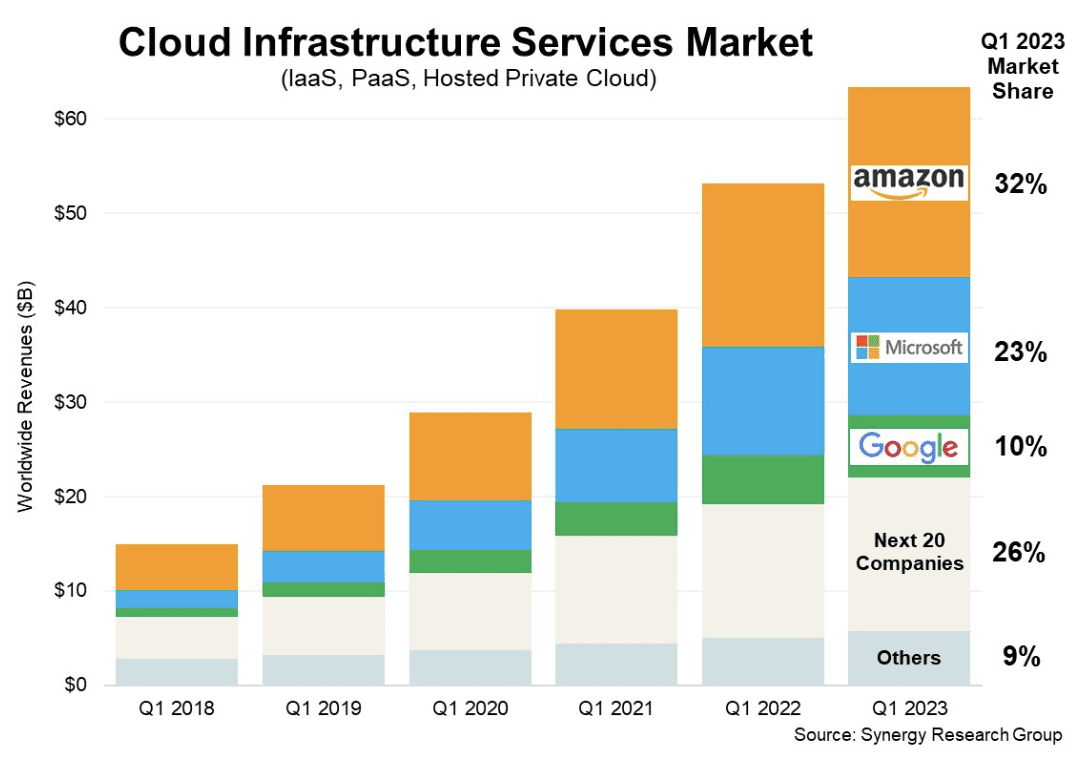
\includegraphics[width=0.9\textwidth]{imagenes/02-marco-teorico/cloud-providers-market-share.png}
  \caption[Distribución del mercado de proveedores de servicios de nube en 2023]{Distribución del mercado de proveedores de servicios de nube en 2023 \cite{john_2023}.}
  \label{fig:cloud-providers-market-share}
\end{figure}

\subsection{Google Cloud Platform}

\textbf{Google Cloud Platform} (GCP) ofrece una serie de productos que permiten
a los usuarios aprovechar la infraestructura interna de Google. Esto incluye
recursos típicos de la nube, como máquinas virtuales bajo demanda y almacenamiento
de objetos, además de APIs para tecnologías avanzadas desarrolladas por Google,
como Bigtable, Cloud Datastore o Kubernetes \cite{geewax2018google}.

A diferencia de otros proveedores de la nube, GCP se distingue por dos razones
principales. Primero, Google ha sido la cuna de tecnologías revolucionarias,
compartidas posteriormente con el mundo a través de publicaciones académicas,
como MapReduce, Bigtable y Spanner. Estas innovaciones, inicialmente exclusivas
de Google, ahora están disponibles para todos. Segundo, la escala de operación
de Google le permite ofrecer precios más bajos gracias a su vasta infraestructura
y hardware personalizado, lo que se traduce en ahorros que benefician al
consumidor, similar a comprar un paquete grande de productos a precio reducido
como en Costco \cite{geewax2018google}. En la Figura \ref{fig:gcp} se muestran
algunos servicios de GCP.

\begin{figure}[!htbp]
  \centering
  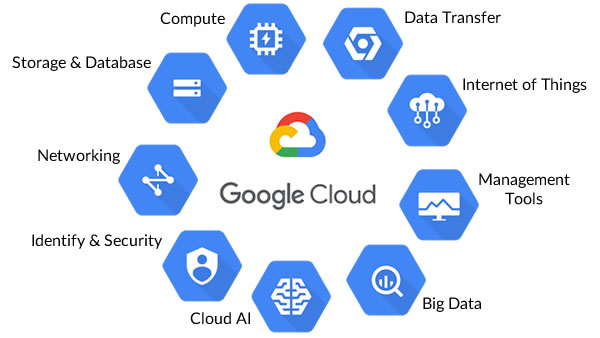
\includegraphics[width=0.6\textwidth]{imagenes/02-marco-teorico/google-cloud-platform-services.jpg}
  \caption[Servicios de Google Cloud Platform]{Servicios de Google Cloud Platform \cite{geewax2018google}.}
  \label{fig:gcp}
\end{figure}

Entre los servicios de GCP que podrían ser relevantes para el desarrollo de
este proyecto se encuentran:

\subsubsection{Cloud DNS}
El servicio de DNS de Google Cloud Platform, Cloud DNS, es un servicio de DNS
escalable, confiable y administrado que permite a los usuarios alojar sus zonas
DNS en la infraestructura de Google. Cloud DNS traduce nombres de dominio como
\texttt{www.example.com} en direcciones IP como \texttt{255.255.255.255}, lo que
permite a los usuarios encontrar recursos en Internet \cite{geewax2018google}.

\subsubsection{Cloud Storage}
Cloud Storage es un servicio de almacenamiento de objetos unificado para desarrolladores
y empresas, que ofrece almacenamiento de objetos altamente escalable y duradero
para cualquier tipo de datos. Es un servicio de almacenamiento de objetos que
permite a los usuarios almacenar y recuperar datos en Google Cloud Platform.
Los objetos de Cloud Storage se almacenan en \textit{buckets}, que son contenedores
de almacenamiento de objetos. Un objeto es un archivo individual que se almacena
en Cloud Storage. Los objetos de Cloud Storage se pueden organizar y controlar
mediante el uso de \textit{etiquetas} \cite{geewax2018google}.

\subsubsection{Cloud CDN}
Cloud CDN es un servicio de red de entrega de contenido que proporciona
distribución de contenido a través de una red global de ubicaciones de
almacenamiento en caché. Cloud CDN reduce la latencia de entrega de contenido,
ahorra ancho de banda y reduce los costos de origen. Cloud CDN se puede habilitar
para cualquier backend que se ejecute en Compute Engine, Google Kubernetes Engine
o Google Cloud Storage \cite{geewax2018google}.

\subsubsection{Cloud Run}
Cloud Run es un servicio administrado que permite ejecutar contenedores sin
estado que se invocan a través de solicitudes HTTP. Cloud Run es un entorno
computacional completamente administrado que se encarga de la escalabilidad
automática, la configuración de la instancia de contenedor y el equilibrio de
carga horizontal. Cloud Run se basa en el proyecto open-source Knative \cite{geewax2018google}.

\subsection{Amazon Web Services}

Amazon Web Services (AWS) es una plataforma de servicios en la nube ampliamente
adoptada que proporciona una variedad de servicios de infraestructura a través de
internet. AWS ofrece una gama extensa de soluciones globales de cómputo,
almacenamiento, bases de datos, análisis, redes y móviles, así como herramientas
de desarrollador, herramientas de gestión, IoT, seguridad y aplicaciones
empresariales \cite{wittig2023amazon}.

Con AWS, las organizaciones pueden desplegar aplicaciones y servicios de manera
rápida y segura, con la flexibilidad de escalar los recursos según sea necesario.
La plataforma está diseñada para ser la más flexible y segura de las plataformas
de computación en la nube, ofreciendo capacidades de cómputo de alto rendimiento
y almacenamiento en la nube, así como bases de datos optimizadas para diferentes
tipos de cargas de trabajo. En la Figura \ref{fig:aws-services} se muestran
algunos servicios de AWS.

\begin{figure}[!htbp]
  \centering
  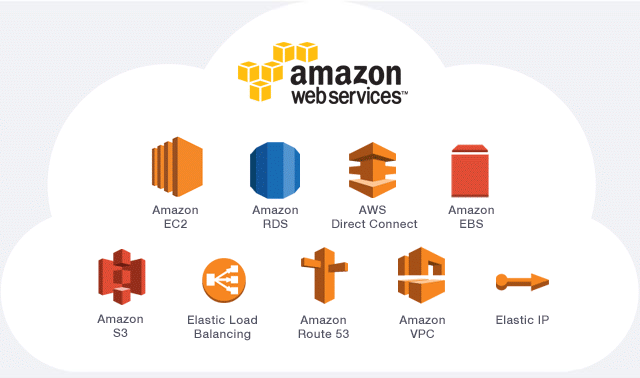
\includegraphics[width=0.6\textwidth]{imagenes/02-marco-teorico/aws-services.png}
  \caption[Servicios de Amazon Web Services]{Servicios de Amazon Web Services \cite{thinkwik_2018_aws}.}
  \label{fig:aws-services}
\end{figure}

AWS es reconocido por su constante innovación y expansión de servicios,
facilitando a empresas de todos los tamaños, desde startups hasta empresas
Fortune 500, la transición hacia la nube y la transformación digital. Su modelo
de pago por uso ayuda a optimizar los costos y a operar infraestructuras más
eficientes \cite{wittig2023amazon}.

Dentro de los servicios de AWS que podrían ser relevantes para el desarrollo de
este proyecto se encuentran:

\subsubsection{Elastic Beanstalk}
AWS Elastic Beanstalk es un servicio que permite a los desarrolladores desplegar
rápidamente y administrar aplicaciones en la nube. Las aplicaciones se pueden
desplegar utilizando una variedad de plataformas, incluyendo Java, .NET, PHP,
Node.js, Python, Ruby, Go y Docker, en servidores web comunes como Apache, Nginx,
Passenger y IIS \cite{thinkwik_2018_aws}.

\subsubsection{ECR}
Amazon Elastic Container Registry (ECR) es un servicio de registro de Docker
totalmente administrado que facilita el almacenamiento, la administración y
la implementación de imágenes de Docker. Los usuarios pueden almacenar,
administrar y desplegar imágenes de Docker en AWS, lo que permite a los
desarrolladores desplegar aplicaciones distribuidas sin necesidad de ejecutar
su propio software de registro de contenedores \cite{thinkwik_2018_aws}.

\subsubsection{S3}
Amazon Simple Storage Service (S3) es un servicio de almacenamiento de objetos
que ofrece escalabilidad, disponibilidad de datos, seguridad y rendimiento
incomparables. S3 es fácil de usar y ofrece una interfaz de servicio web simple
que se puede utilizar para almacenar y recuperar cualquier cantidad de datos,
en cualquier momento y desde cualquier lugar de la web. S3 también ofrece
capacidades de almacenamiento de datos de nivel empresarial para crear,
implementar y escalar aplicaciones, lo que resulta en un acceso rápido y
confiable a los datos y un rendimiento optimizado \cite{cloud2011amazon}.

\subsubsection{Route 53}
Amazon Route 53 es un servicio de sistema de nombres de dominio (DNS) escalable
y altamente disponible. Está diseñado para proporcionar a los desarrolladores
y empresas una forma confiable y rentable de dirigir los usuarios finales a
aplicaciones de Internet, traduciendo nombres de dominio como \texttt{www.example.com}
en direcciones IP como \texttt{255.255.255.0} \cite{cloud2011amazon}.

\subsubsection{CloudFront}
Amazon CloudFront es un servicio de red de entrega de contenido (CDN) rápido,
altamente seguro y programable. CloudFront ofrece una solución de CDN global
y altamente disponible para entregar contenido a través de Internet con baja
latencia y altas velocidades de transferencia de datos. CloudFront funciona
con otros servicios de AWS para proporcionar a los desarrolladores y empresas
una forma fácil de distribuir contenido a los usuarios finales con seguridad,
bajo demanda y con un alto rendimiento \cite{cloud2011amazon}.

\section{GIS}

Los Sistemas de Información Geográfica (GIS) son herramientas computacionales
diseñadas para la adquisición, almacenamiento, análisis y visualización de datos
espaciales. Históricamente, han evolucionado desde la producción de mapas con
enfoques cartográficos tradicionales hacia bases de datos electrónicas flexibles,
permitiendo la superposición de mapas temáticos para resolver conflictos y
relaciones en la gestión del uso del suelo. Los avances técnicos han integrado el
análisis de imágenes de sensores remotos dentro de las prácticas estándar de GIS,
superando la división entre datos en formato \textit{raster} y \textit{vector}. En
la actualidad, los GIS comerciales ofrecen capacidades ampliadas para trabajar con
ambos tipos de datos y han incluido lenguajes de programación internos que amplían
su aplicación a modelos ambientales variados, aunque tradicionalmente han ignorado
aspectos como la incertidumbre y la variabilidad espacio-temporal en favor de la
precisión geométrica \cite{burrough2001gis}.

En la Figura \ref{fig:gis-analysis} se muestra un ejemplo de las aplicaciones de
los GIS en el análisis de datos espaciales, en este caso, aplicado a una imagen
satelital y cómo se puede descomponer la información en diferentes capas.

\begin{figure}[!htbp]
  \centering
  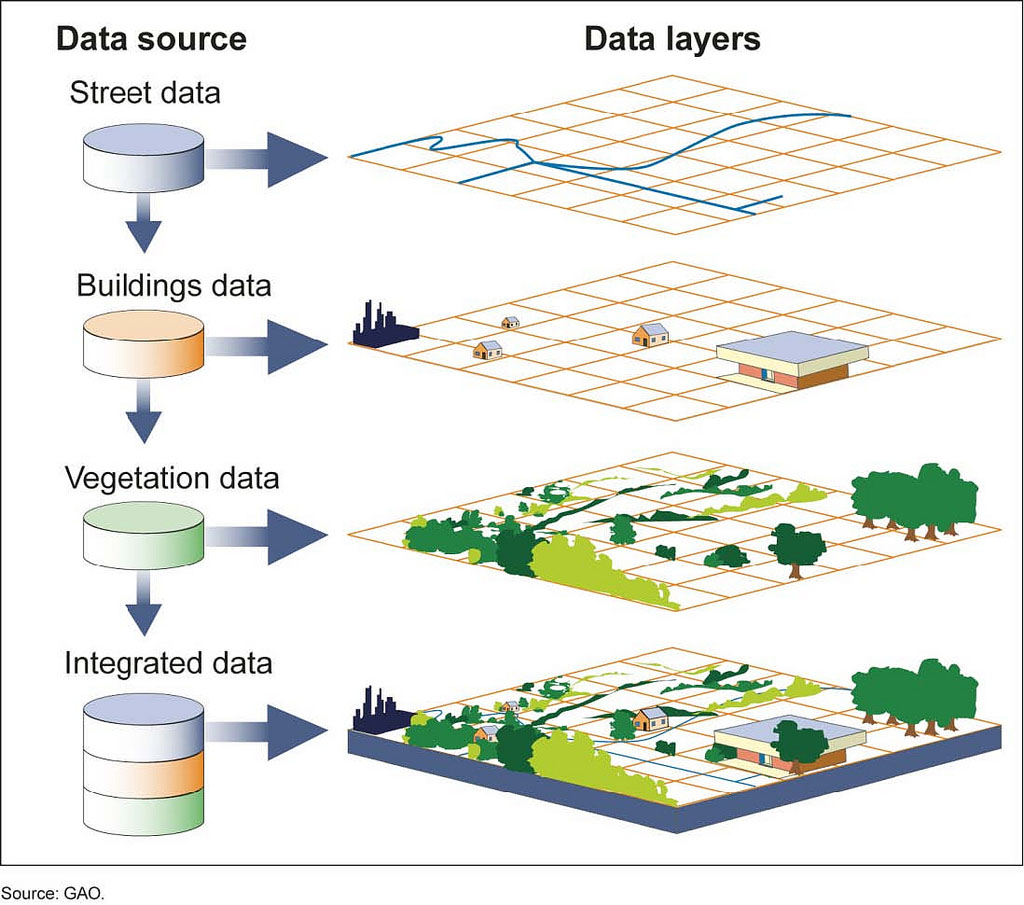
\includegraphics[width=0.9\textwidth]{imagenes/02-marco-teorico/gis-analysis.jpg}
  \caption[Aplicaciones de los GIS en el análisis de datos espaciales]{Aplicaciones de los GIS en el análisis de datos espaciales \cite{national_geographic_gis_2023}.}
  \label{fig:gis-analysis}
\end{figure}

La valuación inmobiliaria es una de las aplicaciones más comunes de los GIS,
permitiendo la visualización de datos espaciales y la generación de mapas temáticos
para la toma de decisiones. Los GIS también se utilizan para la planificación urbana,
la gestión de recursos naturales, la gestión de desastres, la gestión de infraestructura
y el análisis de redes, entre otros \cite{wyatt1997development}.

Existen múltiples software GIS, tanto comerciales como de código abierto, que
permiten la visualización y análisis de datos espaciales. A continuación se
abordarán algunos de los más utilizados.

\subsection{QGIS}
QGIS es un sistema de información geográfica (SIG) de código abierto que comenzó
en 2002 y opera en plataformas Unix, Windows y macOS. Desarrollado con Qt y C++,
ofrece una interfaz de usuario amigable, además de aplicaciones para dispositivos
móviles. Inicialmente un visor de datos SIG, ahora QGIS es utilizado para
visualización de datos GIS, captura de datos, análisis avanzado y presentaciones
en mapas. Admite numerosos formatos de datos y se expande fácilmente con complementos.
Publicado bajo la Licencia Pública General GNU (GPL), QGIS es gratuito y de código
fuente abierto, asegurando acceso y modificación libres \cite{qgis_3.28_user_guide}.

En la Figura \ref{fig:qgis-screenshot} se muestra la interfaz de usuario de QGIS.

\begin{figure}[!htbp]
  \centering
  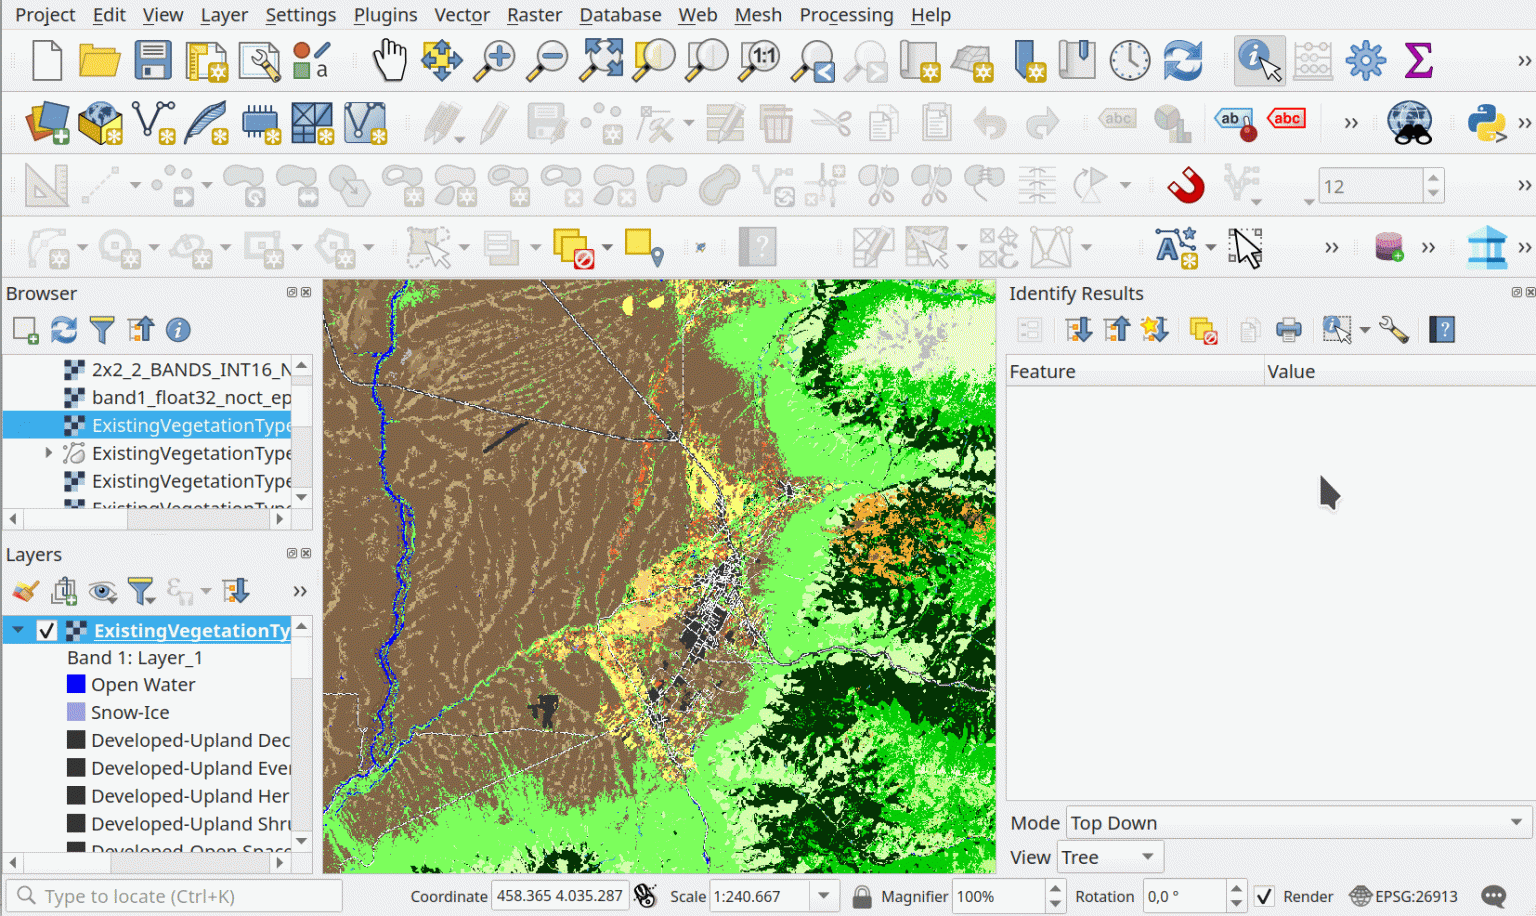
\includegraphics[width=0.9\textwidth]{imagenes/02-marco-teorico/qgis-screenshot.png}
  \caption[Interfaz de usuario de QGIS]{Interfaz de usuario de QGIS \cite{alonso_2023_qgis}.}
  \label{fig:qgis-screenshot}
\end{figure}

\subsection{kepler.gl}
Kepler.gl es una aplicación web de alto rendimiento y agnóstica a los datos,
diseñada para la exploración visual de conjuntos de datos geolocalizados a gran
escala. Como herramienta de \textit{GIS}, kepler.gl se destaca por su capacidad
de renderizar millones de puntos, representando miles de trayectos y realizando
agregaciones espaciales al vuelo. Construido sobre tecnologías robustas como
Mapbox GL y deck.gl, kepler.gl es una potente plataforma para analizar y visualizar
datos espaciales en una variedad de formas, facilitando la comprensión de patrones
y tendencias complejas. Además, kepler.gl funciona como un componente de React que
utiliza Redux para la gestión de su estado y flujo de datos, lo que permite su
integración y personalización en otras aplicaciones basadas en React-Redux,
ofreciendo así una solución versátil para el análisis de datos geoespaciales en el
ámbito del \textit{GIS} \cite{kepler_gl_docs}.

En la Figura \ref{fig:kepler-gl} se muestra la interfaz de usuario de kepler.gl.

\begin{figure}[!htbp]
  \centering
  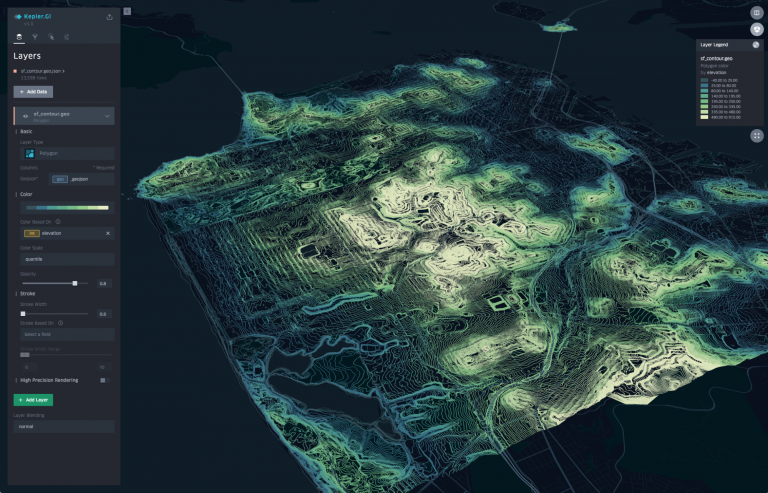
\includegraphics[width=0.9\textwidth]{imagenes/02-marco-teorico/kepler-demo.png}
  \caption[Interfaz de usuario de kepler.gl]{Interfaz de usuario de kepler.gl \cite{kepler_gl_docs}.}
  \label{fig:kepler-gl}
\end{figure}

\subsection{Google Maps}
Google Maps es un servicio de mapeo web proporcionado por Google. Ofrece imágenes
satelitales, fotografías aéreas, mapas de calles, vistas panorámicas de calles
(Street View), condiciones de tráfico en tiempo real, y planificación de rutas
para viajar a pie, en coche, bicicleta y transporte público. Desde su lanzamiento
en 2005, Google Maps se ha convertido en una de las herramientas más utilizadas
y avanzadas en su categoría, facilitando la exploración y navegación por todo el
mundo a millones de usuarios \cite{google_maps_platform_start}. En la Figura
\ref{fig:google-maps-screenshot} se muestra la interfaz de usuario de Google Maps.

\begin{figure}[!htbp]
  \centering
  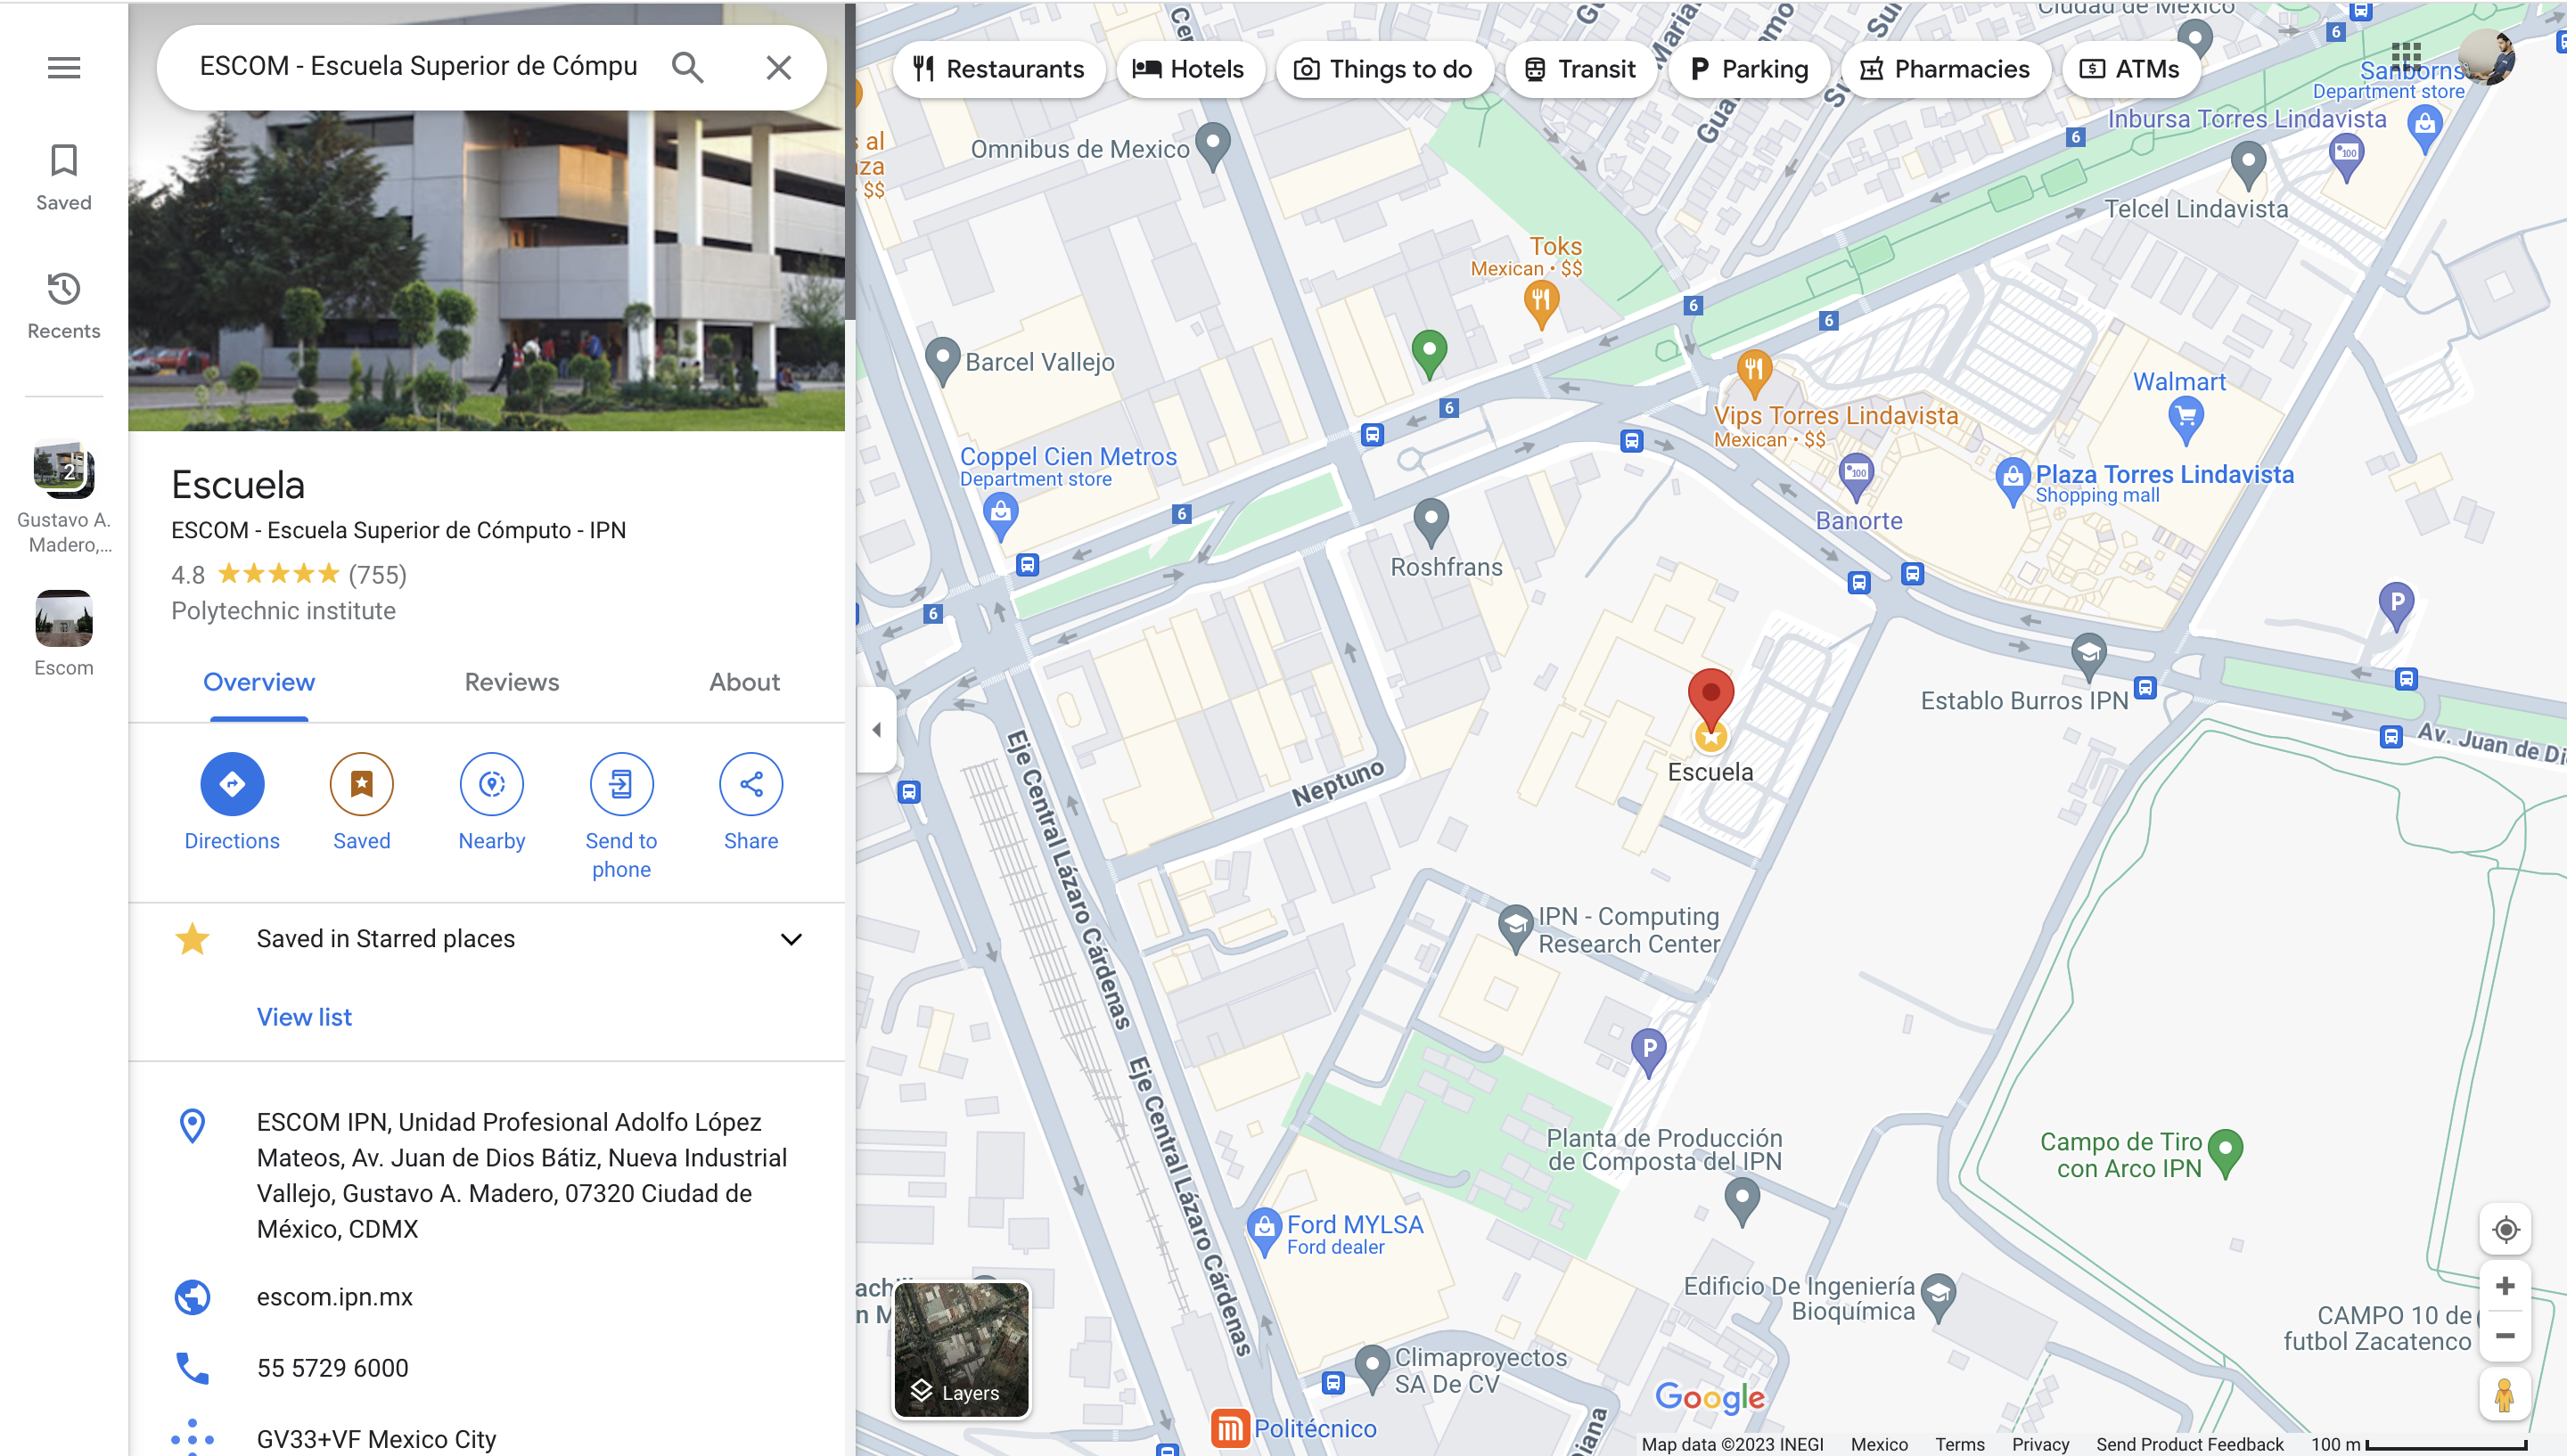
\includegraphics[width=0.9\textwidth]{imagenes/02-marco-teorico/google-maps-screenshot.png}
  \caption[Interfaz de usuario de Google Maps]{Interfaz de usuario de Google Maps.}
  \label{fig:google-maps-screenshot}
\end{figure}

Dentro de los servicios que ofrece, los más relevantes para el desarrollo de este
proyecto son:

\subsubsection{API de Mapas}

La API de Google Maps permite a los desarrolladores integrar los servicios de
mapeo de Google en sus propias aplicaciones y sitios web. Esta API ofrece una
amplia gama de funcionalidades, como la visualización de mapas personalizados,
la superposición de datos, y la manipulación de elementos del mapa. Los
desarrolladores pueden utilizar esta API para mostrar mapas interactivos y
dinámicos, con soporte para diferentes tipos de visualización como mapas de
carreteras, imágenes satelitales y terrenos. También es posible personalizar
los mapas para que se ajusten al estilo y necesidades específicas de la aplicación
o sitio web \cite{google_maps_platform_start}.

\subsubsection{API de Reverse Geocoding}

La API de Reverse Geocoding de Google Maps es otra herramienta poderosa para
los desarrolladores. Permite convertir coordenadas geográficas (latitud y longitud)
en direcciones postales o nombres de lugares. Esta funcionalidad es particularmente
útil para aplicaciones que necesitan determinar la ubicación física exacta a partir
de coordenadas GPS. La API proporciona respuestas detalladas, incluyendo el nombre
del lugar, la dirección, el barrio y otros datos relevantes. Esto es ampliamente
utilizado en aplicaciones de logística, viajes, y servicios basados en ubicación
para mejorar la experiencia del usuario al proporcionar información contextual
sobre su ubicación actual \cite{google_geocoding_2023}.


